\documentclass{beamer}
% \documentclass[handout]{beamer}

\usepackage{amsmath,amsfonts,amsthm,amssymb,euscript,mathrsfs,url,stmaryrd,bbm}
\usepackage{subfigure}
\usepackage{tikz}

\usepackage{color}
\usepackage{import}

% \usepackage[absolute,overlay]{textpos}

\usepackage[utf8]{inputenc}

% should get rid of superfluous equation labels
% or all labels, if we never reference
\usepackage{mathtools}
\mathtoolsset{showonlyrefs}

\usepackage{multicol}
\usepackage{multirow}
\usepackage{colortbl}
\usepackage{booktabs}

% \usepackage[export]{adjustbox}% http://ctan.org/pkg/adjustbox


% theme
\usetheme{Singapore}
\useinnertheme{rounded}
\usecolortheme{rose}
% usetheme{Warsaw}

%farbversuche
%sieht sehr gut aus aber erstmal nicht
\definecolor{grey}{RGB}{0,0,0}
%aber wir machen erstmal was anderes
\definecolor{darkgreen}{RGB}{90,160,70}
\definecolor{darkred}{RGB}{160,70,70}
\definecolor{brickred}{RGB}{220,55,75}
% \definecolor{yellow}{RGB}{255,255,0}
\definecolor{turquoise}{RGB}{0,255,255}
% \definecolor{grey}{RGB}{0,255,255}
\definecolor{maroon}{RGB}{128,0,0}

%farbe als structure setzen
\setbeamercolor{structure}{fg=maroon!40!black}
% \setbeamercolor{structure}{fg=white!72!black}
%\setbeamercolor{structure}{fg=white!50!green!60!black}

%versuch die textfarbe zu setzen
% \setbeamercolor{normal text}{fg=blue!30!black}
%\setbeamercolor{normal text}{fg=blue}

% cover up
\setbeamercovered{transparent}

% make it work on matthias' laptop
% \setbeamertemplate{blocks}[default]


% macros
\renewcommand{\P}{\mathbb{P}}
\newcommand{\E}{\mathbb{E}}
\newcommand{\V}{\mathbb{V}}
% \newcommand{\N}{\ensuremath{\mathbb{N}}}
\newcommand{\R}{\ensuremath{\mathbb{R}}}
\newcommand{\1}{\ensuremath{\mathbf{1}}}
% \input{macros.tex}


% \newlength{\nodedist}


\setbeamercolor*{title}{use=structure,fg=white,bg=structure.fg,}
\setbeamertemplate{title page}[default][colsep=-4bp,rounded=true,shadow=true]

%we need this because sometimes we flip it
\def\defaultbeameritem{ball}
\setbeamertemplate{itemize items}[\defaultbeameritem]


% fancy footline
\setbeamertemplate{footline}
{

\begin{tikzpicture}(0,0)
\draw[draw=none,top color=white,bottom color=grey!20!white] (0,0) rectangle (\paperwidth,0.25);
% \node at (\paperwidth-12,0.2) {\insertframenumber /\inserttotalframenumber};
\node at (\paperwidth-12,0.2) {\insertpagenumber /\insertpresentationendpage};
\end{tikzpicture}}

%suppress navigation symbols
\setbeamertemplate{navigation symbols}{}
% % no footline
% \setbeamertemplate{footline}{}
% \setbeamertemplate{footline}[frame number]

% we want numbered figures
\setbeamertemplate{caption}[numbered]

% relevant stuff
\title{EMBO PopGen}
\subtitle{Introduction to population genetics}
\author{Matthias Steinrücken\\[2ex]{\scriptsize adapted from Matteo Fumagalli (EMBO, 2024)}}
% \institute{Department of Ecology and Evolution, University of Chicago\\ Department of Human Genetics, University of Chicago\\ NITMB} 
\institute{Department of Ecology and Evolution, University of Chicago\\ Department of Human Genetics, University of Chicago} 
\date{Day 2a, June 24, 2025}

\def\newblock{\hskip .11em plus .33em minus .07em}
\renewcommand{\raggedright}{\leftskip=0pt \rightskip=0pt plus 0cm} 
\renewcommand{\insertnavigation}[1]{\insertsectionnavigationhorizontal{#1}{}{}}



\begin{document}
%%%%%%%%%%%%%%%%%%%%%%%%%%%%%%%%%%%%%%%%%%%%%%%%%%%%%%%%%%%%%%%%%%%%%%%%%%%%%%%%%%%%%%
%
%
%
%%%%%%%%%%%%%%%%%%%%%%%%%%%%%%%%%%%%%%%%%%%%%%%%%%%%%%%%%%%%%%%%%%%%%%%%%%%%%%%%%%%%%%
\logo{\begin{minipage}[!b]{2cm}
\includegraphics[width=1.5cm]{graphics_day2a_popgen/university.seal.rgb.maroon.png}\\\phantom{a}\\\phantom{b}\end{minipage}}
%%%%%%%%%%%%%%%%%%%%%%%%%%%%%%%%%%%%%%%%%%%%%%%%%%%%%%%%%%%%%%%%%%%%%%%%%%%%%%%%%%%%%%
%
%
%
%%%%%%%%%%%%%%%%%%%%%%%%%%%%%%%%%%%%%%%%%%%%%%%%%%%%%%%%%%%%%%%%%%%%%%%%%%%%%%%%%%%%%%
\begin{frame}
	\titlepage 
	% \addtocounter{framenumber}{-1}
\end{frame}
\logo{}
%%%%%%%%%%%%%%%%%%%%%%%%%%%%%%%%%%%%%%%%%%%%%%%%%%%%%%%%%%%%%%%%%%%%%%%%%%%%%%%%%%%%%%
%
%
%
%%%%%%%%%%%%%%%%%%%%%%%%%%%%%%%%%%%%%%%%%%%%%%%%%%%%%%%%%%%%%%%%%%%%%%%%%%%%%%%%%%%%%%
\begin{frame}\frametitle{Intended Learning Outcomes}
	In this session you will learn:
	\begin{itemize}
		\item To describe all different types of genetic data.
		\item To demonstrate the relationship between allele and genotype frequencies.
		\item To calculate Hardy-Weinberg Equilibrium proportions.
	\end{itemize}
\end{frame}
%%%%%%%%%%%%%%%%%%%%%%%%%%%%%%%%%%%%%%%%%%%%%%%%%%%%%%%%%%%%%%%%%%%%%%%%%%%%%%%%%%%%%%
%
%
%
%%%%%%%%%%%%%%%%%%%%%%%%%%%%%%%%%%%%%%%%%%%%%%%%%%%%%%%%%%%%%%%%%%%%%%%%%%%%%%%%%%%%%%
\begin{frame}\frametitle{Terminology}
	Before we dive into the genetic basis of evolution, let us define some important terms, such as:
	\begin{itemize}
		\item Gene
		\item Phenotype
		\item Locus
		\item Allele
		\item Genotype
		\item Haplotype
	\end{itemize}
\end{frame}
%%%%%%%%%%%%%%%%%%%%%%%%%%%%%%%%%%%%%%%%%%%%%%%%%%%%%%%%%%%%%%%%%%%%%%%%%%%%%%%%%%%%%%
%
%
%
%%%%%%%%%%%%%%%%%%%%%%%%%%%%%%%%%%%%%%%%%%%%%%%%%%%%%%%%%%%%%%%%%%%%%%%%%%%%%%%%%%%%%%
\begin{frame}\frametitle{Gene}
	A gene can be defined as:
	\begin{itemize}
		\item The segregating and heritable determinant of the phenotype$^{*}$.
		\item The fundamental physical and functional unit of heredity, which carries information from one generation to the next one.
		\item A segment of DNA, composed of a transcribed region and regulatory sequences that make possible transcription and regulation.
	\end{itemize}
	 \vspace{1ex}{\small $^{*}$A trait or characteristic of the individual carrier (more on this later).}
\end{frame}
%%%%%%%%%%%%%%%%%%%%%%%%%%%%%%%%%%%%%%%%%%%%%%%%%%%%%%%%%%%%%%%%%%%%%%%%%%%%%%%%%%%%%%
%
%
%
%%%%%%%%%%%%%%%%%%%%%%%%%%%%%%%%%%%%%%%%%%%%%%%%%%%%%%%%%%%%%%%%%%%%%%%%%%%%%%%%%%%%%%
\begin{frame}\frametitle{Gene}
	For example, the human \emph{LCT} gene ``provides instructions for making an enzyme called lactase. This enzyme helps to digest lactose, a sugar found in milk and other dairy products$^{*}$''.
	\begin{figure}
	\begin{center}
		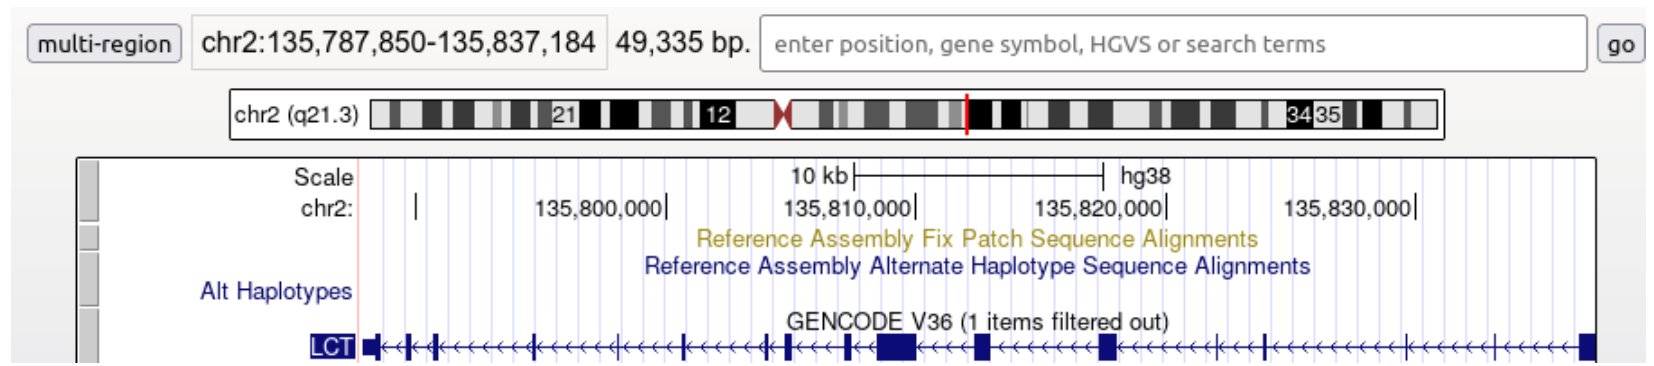
\includegraphics[width=\textwidth]{graphics_day2a_popgen/lct_region.png}
	\end{center}
	\caption{\emph{LCT} gene is located on chromosome 2 in the human genome and spans approx. 50k base pairs.}
	\end{figure}
	 {\small $^{*}$https://pubchem.ncbi.nlm.nih.gov/gene/LCT/human}
\end{frame}
%%%%%%%%%%%%%%%%%%%%%%%%%%%%%%%%%%%%%%%%%%%%%%%%%%%%%%%%%%%%%%%%%%%%%%%%%%%%%%%%%%%%%%
%
%
%
%%%%%%%%%%%%%%%%%%%%%%%%%%%%%%%%%%%%%%%%%%%%%%%%%%%%%%%%%%%%%%%%%%%%%%%%%%%%%%%%%%%%%%
\begin{frame}\frametitle{Phenotype}
	A \textbf{phenotype} can be defined as a physical/behavioral (etc.) characteristic of an individual.\\[3ex]
	\begin{block}{}
		The genetic component of the phenotype is heritable.
	\end{block}
\end{frame}
%%%%%%%%%%%%%%%%%%%%%%%%%%%%%%%%%%%%%%%%%%%%%%%%%%%%%%%%%%%%%%%%%%%%%%%%%%%%%%%%%%%%%%
%
%
%
%%%%%%%%%%%%%%%%%%%%%%%%%%%%%%%%%%%%%%%%%%%%%%%%%%%%%%%%%%%%%%%%%%%%%%%%%%%%%%%%%%%%%%
\begin{frame}\frametitle{Phenotype}
	For example, ``lactase is the enzyme that carries out the digestion of the milk sugar lactose. Its expression decreases at some point after the weaning period is over in most mammals and in around 68\% of all living adult humans. However, in some humans, particularly those from populations with a history of dairying, lactase is expressed throughout adulthood. This phenotype is called lactase persistence''$^{*}$.\\[2ex]
	 {\small $^{*}$https://pubmed.ncbi.nlm.nih.gov/24861860/}
\end{frame}
%%%%%%%%%%%%%%%%%%%%%%%%%%%%%%%%%%%%%%%%%%%%%%%%%%%%%%%%%%%%%%%%%%%%%%%%%%%%%%%%%%%%%%
%
%
%
%%%%%%%%%%%%%%%%%%%%%%%%%%%%%%%%%%%%%%%%%%%%%%%%%%%%%%%%%%%%%%%%%%%%%%%%%%%%%%%%%%%%%%
\begin{frame}\frametitle{Lactase persistence}
	\begin{figure}
	\begin{center}
		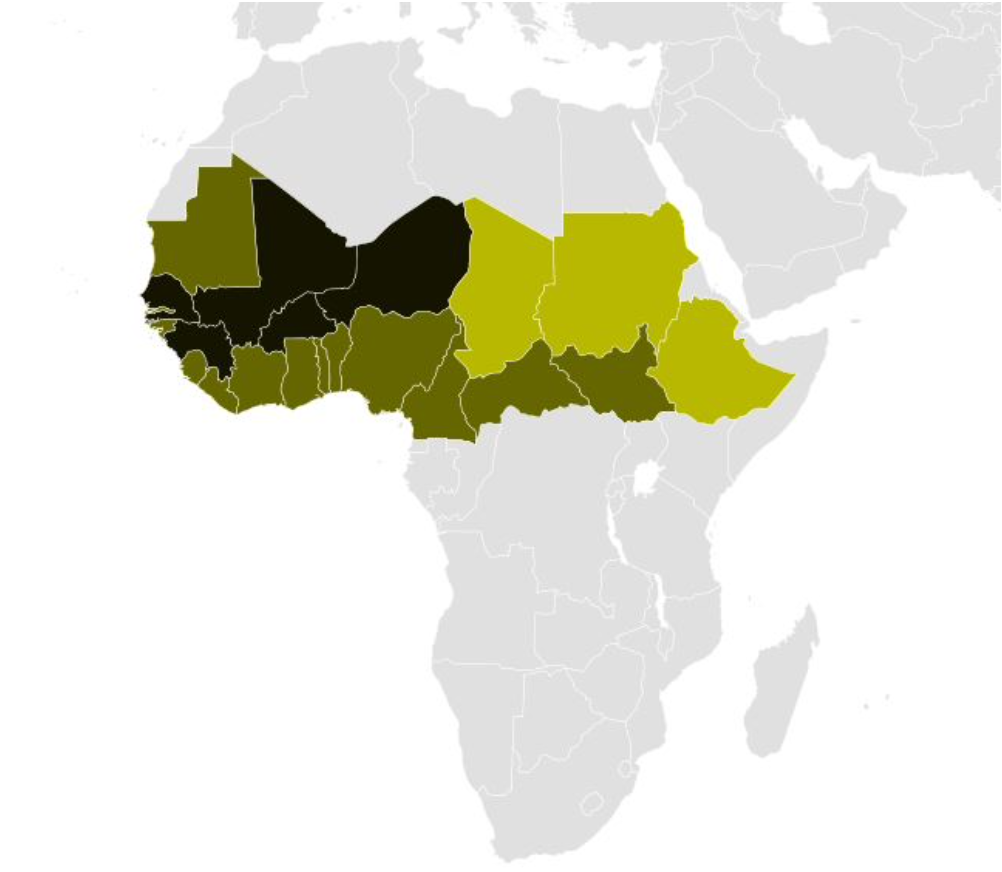
\includegraphics[width=.5\textwidth]{graphics_day2a_popgen/africa_map_fula.png}
	\end{center}
	\caption{A geographical distribution map of Fula people who show high prevalence of lactase persistence.}
	\end{figure}
	 {\scriptsize \url{https://www.sciencedirect.com/science/article/pii/S0002929714000676}}
\end{frame}
%%%%%%%%%%%%%%%%%%%%%%%%%%%%%%%%%%%%%%%%%%%%%%%%%%%%%%%%%%%%%%%%%%%%%%%%%%%%%%%%%%%%%%
%
%
%
%%%%%%%%%%%%%%%%%%%%%%%%%%%%%%%%%%%%%%%%%%%%%%%%%%%%%%%%%%%%%%%%%%%%%%%%%%%%%%%%%%%%%%
\begin{frame}\frametitle{Types of genetic data}
	The study of the genetic basis of evolution is applicable to all genetic \emph{variants} that can be distinguished by some means and that can be \emph{transmitted} from parents to offspring.\\[2ex]
	Any variants with these properties are called \textbf{alleles}:
	\begin{itemize}
		\item Single nucleotide polymorphism
		\item Insertion/deletion
		\item Microsatellites
	\end{itemize}
\end{frame}
%%%%%%%%%%%%%%%%%%%%%%%%%%%%%%%%%%%%%%%%%%%%%%%%%%%%%%%%%%%%%%%%%%%%%%%%%%%%%%%%%%%%%%
%
%
%
%%%%%%%%%%%%%%%%%%%%%%%%%%%%%%%%%%%%%%%%%%%%%%%%%%%%%%%%%%%%%%%%%%%%%%%%%%%%%%%%%%%%%%
\begin{frame}\frametitle{Single nucleotide polymorphism (SNP)}
	\begin{figure}
	\begin{center}
		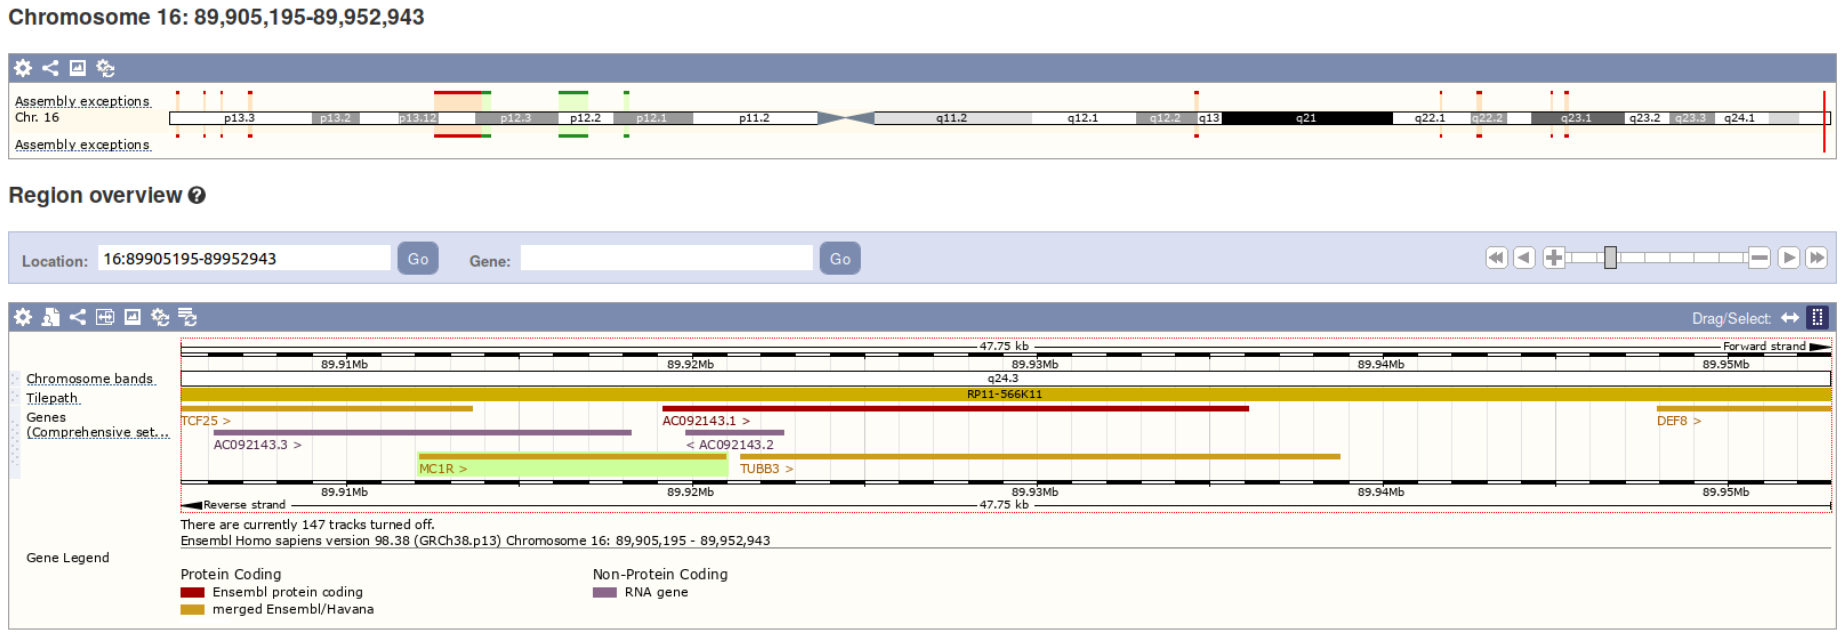
\includegraphics[width=.85\textwidth]{graphics_day2a_popgen/mc1r_human_gene.png}
	\end{center}
	\caption{\emph{MC1R} human gene.}
	\end{figure}
	The \texttt{C}/\texttt{T} variation at position 478 in \emph{MC1R} is an example of a \textbf{single nucleotide polymorphism} (SNP, ``snip'').
\end{frame}
%%%%%%%%%%%%%%%%%%%%%%%%%%%%%%%%%%%%%%%%%%%%%%%%%%%%%%%%%%%%%%%%%%%%%%%%%%%%%%%%%%%%%%
%
%
%
%%%%%%%%%%%%%%%%%%%%%%%%%%%%%%%%%%%%%%%%%%%%%%%%%%%%%%%%%%%%%%%%%%%%%%%%%%%%%%%%%%%%%%
\begin{frame}\frametitle{Single nucleotide polymorphism (SNP)}
	MC1R codes for a protein called melanocortin 1 receptor.
	\begin{columns}
	\begin{column}{.4\textwidth}
		\begin{figure}
		\begin{center}
			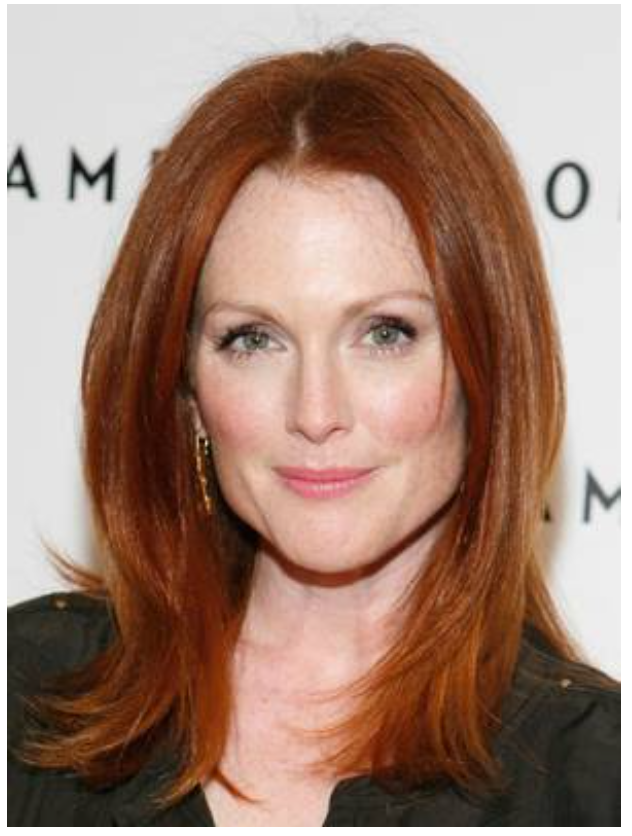
\includegraphics[width=.65\textwidth]{graphics_day2a_popgen/julianne_moore.png}
		\end{center}
		\caption{Julianne Moore.}
		\end{figure}
	\end{column}
	\begin{column}{.6\textwidth}
		Individuals with two copies of \texttt{T} allele in position 478 of the gene \emph{MC1R} tend to have freckles and red hair.\\[2ex]
		This mutation disrupts the protein and causes an increase of the production of red/yellow pigment melanin instead of brown/black.
	\end{column}
	\end{columns}
	{\tiny Please be aware that most phenotypes are not fully determined by the presence of a single genotype only.}
\end{frame}
%%%%%%%%%%%%%%%%%%%%%%%%%%%%%%%%%%%%%%%%%%%%%%%%%%%%%%%%%%%%%%%%%%%%%%%%%%%%%%%%%%%%%%
%
%
%
%%%%%%%%%%%%%%%%%%%%%%%%%%%%%%%%%%%%%%%%%%%%%%%%%%%%%%%%%%%%%%%%%%%%%%%%%%%%%%%%%%%%%%
\begin{frame}\frametitle{Insertion / deletion (indel)}
	An \textbf{indel} is the insertion or deletion of few nucleotides.
	\begin{columns}
	\begin{column}{.4\textwidth}
		\begin{figure}
		\begin{center}
			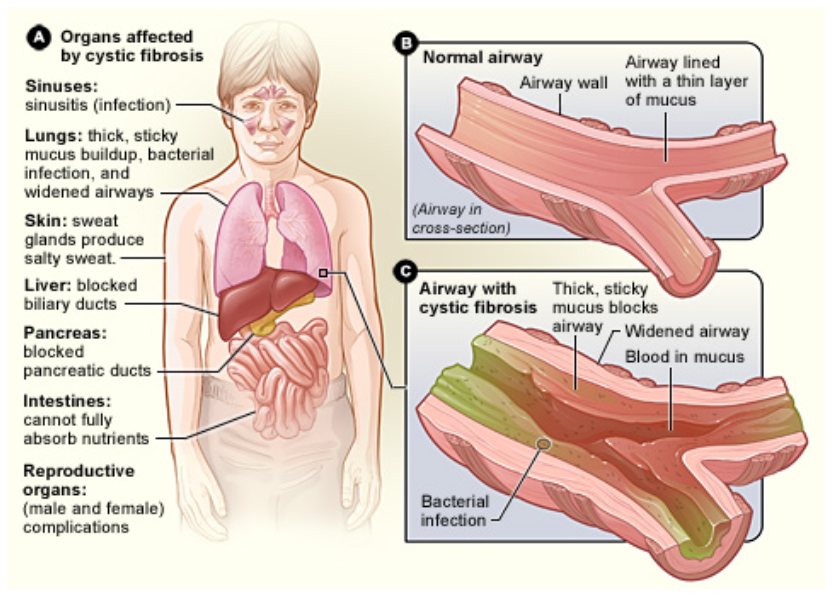
\includegraphics[width=.85\textwidth]{graphics_day2a_popgen/cystic_fibrosis.png}
		\end{center}
		\caption{Cystic fibrosis.}
		\end{figure}
	\end{column}
	\begin{column}{.6\textwidth}
		The \emph{CFTR} gene codes for a transmembrane protein involved in osmotic balance of cells.\\[2ex]
		Variant \texttt{$\Delta$F508} has a three-base deletion that results in the absence of the 508th amino acid phenylanine (F).
	\end{column}
	\end{columns}
\end{frame}
%%%%%%%%%%%%%%%%%%%%%%%%%%%%%%%%%%%%%%%%%%%%%%%%%%%%%%%%%%%%%%%%%%%%%%%%%%%%%%%%%%%%%%
%
%
%
%%%%%%%%%%%%%%%%%%%%%%%%%%%%%%%%%%%%%%%%%%%%%%%%%%%%%%%%%%%%%%%%%%%%%%%%%%%%%%%%%%%%%%
\begin{frame}\frametitle{Microsatellites}
	DNA replication machinery tends to miscopy repeated sequences in the genome.
	\begin{columns}
	\begin{column}{.32\textwidth}
		\begin{figure}
		\begin{center}
			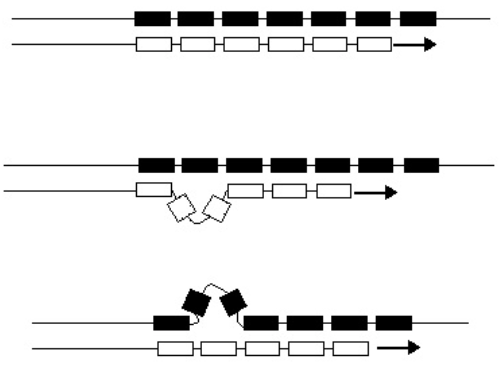
\includegraphics[width=.85\textwidth]{graphics_day2a_popgen/dna_replication_errors.png}
		\end{center}
		\caption{DNA replication errors.}
		\end{figure}
	\end{column}
	\begin{column}{.68\textwidth}
		E.g. sequence \texttt{AGCTGCACACACACACACATGCTG} has \texttt{CA} motif repeated seven times, while other individuals may have a different number of copies, thus $(\texttt{CA})_n$.\\[2ex]
		Simple sequence repeats (SSRs) or \textbf{microsatellites} are variants on the number of repeats transmitted during meiosis, with a small possibility of error.
	\end{column}
	\end{columns}
\end{frame}
%%%%%%%%%%%%%%%%%%%%%%%%%%%%%%%%%%%%%%%%%%%%%%%%%%%%%%%%%%%%%%%%%%%%%%%%%%%%%%%%%%%%%%
%
%
%
%%%%%%%%%%%%%%%%%%%%%%%%%%%%%%%%%%%%%%%%%%%%%%%%%%%%%%%%%%%%%%%%%%%%%%%%%%%%%%%%%%%%%%
\begin{frame}\frametitle{Terminology}
	Let’s introduce some additional concepts that deal with how genetic variation can be summarized. These are:
	\begin{itemize}
		\item \textbf{Allele}: A distinguishable and heritable quantity (SNP, indel, microsat).
		\item \textbf{Locus}: Any position (or unit) in the genome with one or more alleles.
		\item \textbf{Genotype}: Combination of alleles carried by an individual at a particular locus.
	\end{itemize}
	\begin{block}{Example}
		An individual has \texttt{A} and \texttt{G} alleles, and therefore has \texttt{A/G} genotype, at locus in position 8,789,654 of chromosome 1.
	\end{block}
\end{frame}
%%%%%%%%%%%%%%%%%%%%%%%%%%%%%%%%%%%%%%%%%%%%%%%%%%%%%%%%%%%%%%%%%%%%%%%%%%%%%%%%%%%%%%
%
%
%
%%%%%%%%%%%%%%%%%%%%%%%%%%%%%%%%%%%%%%%%%%%%%%%%%%%%%%%%%%%%%%%%%%%%%%%%%%%%%%%%%%%%%%
\begin{frame}\frametitle{Locus}
	A \textbf{locus} (pl. \emph{loci}) can be defined as a generic position on a chromosome, or the position on a chromosome of a gene or other chromosome marker. Generally speaking, a locus is a location.
\end{frame}
%%%%%%%%%%%%%%%%%%%%%%%%%%%%%%%%%%%%%%%%%%%%%%%%%%%%%%%%%%%%%%%%%%%%%%%%%%%%%%%%%%%%%%
%
%
%
%%%%%%%%%%%%%%%%%%%%%%%%%%%%%%%%%%%%%%%%%%%%%%%%%%%%%%%%%%%%%%%%%%%%%%%%%%%%%%%%%%%%%%
\begin{frame}\frametitle{Locus}
	\begin{figure}
	\begin{center}
		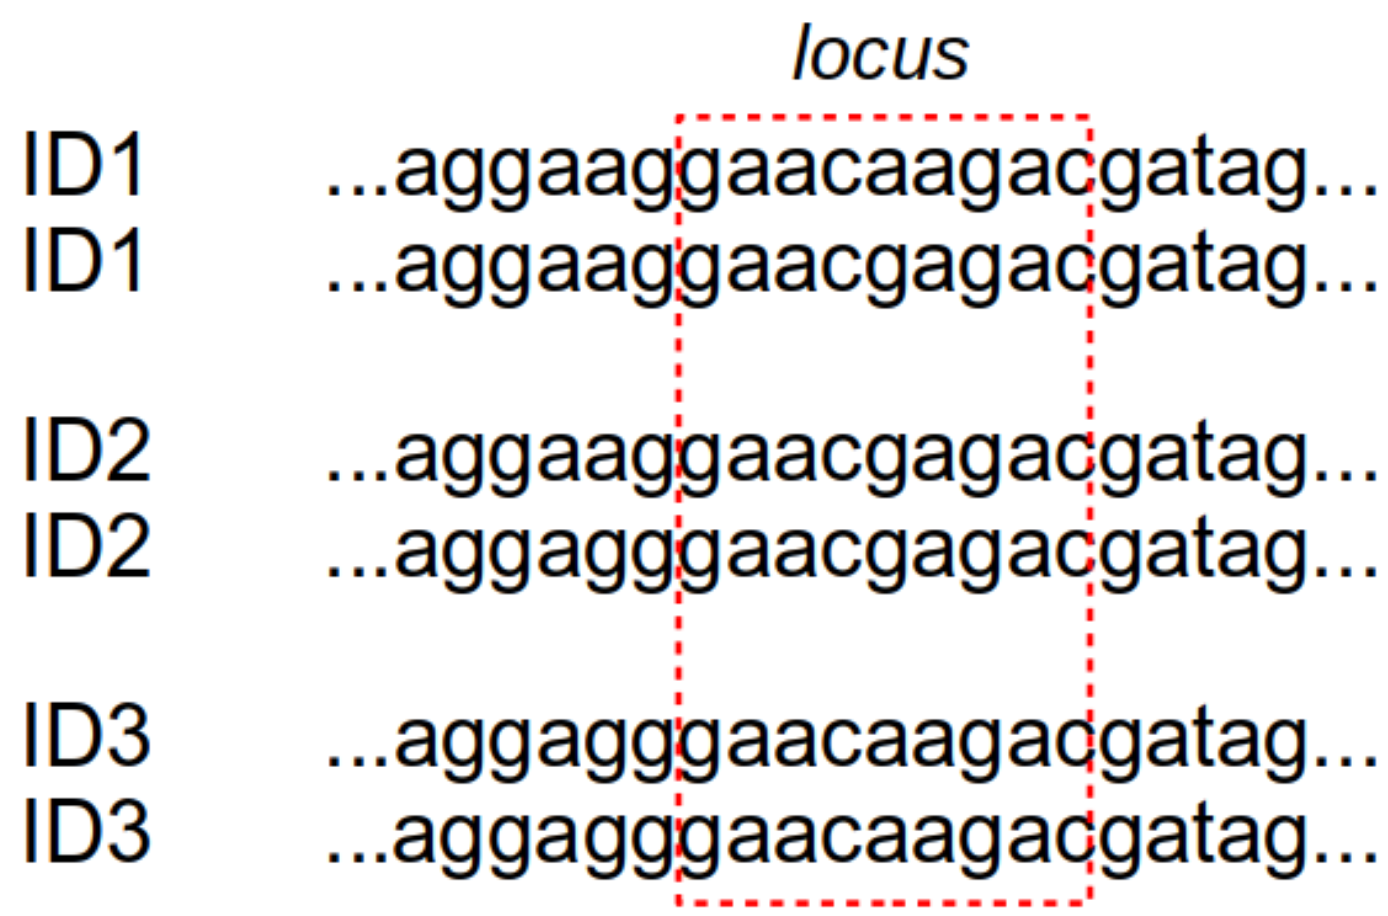
\includegraphics[width=.6\textwidth]{graphics_day2a_popgen/locus_example.png}
	\end{center}
	\caption{A \emph{locus} of nine base pairs (bp).}
	\end{figure}
\end{frame}
%%%%%%%%%%%%%%%%%%%%%%%%%%%%%%%%%%%%%%%%%%%%%%%%%%%%%%%%%%%%%%%%%%%%%%%%%%%%%%%%%%%%%%
%
%
%
%%%%%%%%%%%%%%%%%%%%%%%%%%%%%%%%%%%%%%%%%%%%%%%%%%%%%%%%%%%%%%%%%%%%%%%%%%%%%%%%%%%%%%
\begin{frame}\frametitle{Allele}
	An \textbf{allele} is a variant of a gene or locus. Different alleles can lead to different phenotypes.\\[2ex]
	As we will see later, diploids have two copies of each gene. Therefore, we define as \emph{homozygote} an individual that possesses two copies of the same allele, while as \emph{heterozygote} if it possesses two different alleles.
\end{frame}
%%%%%%%%%%%%%%%%%%%%%%%%%%%%%%%%%%%%%%%%%%%%%%%%%%%%%%%%%%%%%%%%%%%%%%%%%%%%%%%%%%%%%%
%
%
%
%%%%%%%%%%%%%%%%%%%%%%%%%%%%%%%%%%%%%%%%%%%%%%%%%%%%%%%%%%%%%%%%%%%%%%%%%%%%%%%%%%%%%%
\begin{frame}\frametitle{Allele}
	\begin{figure}
	\begin{center}
		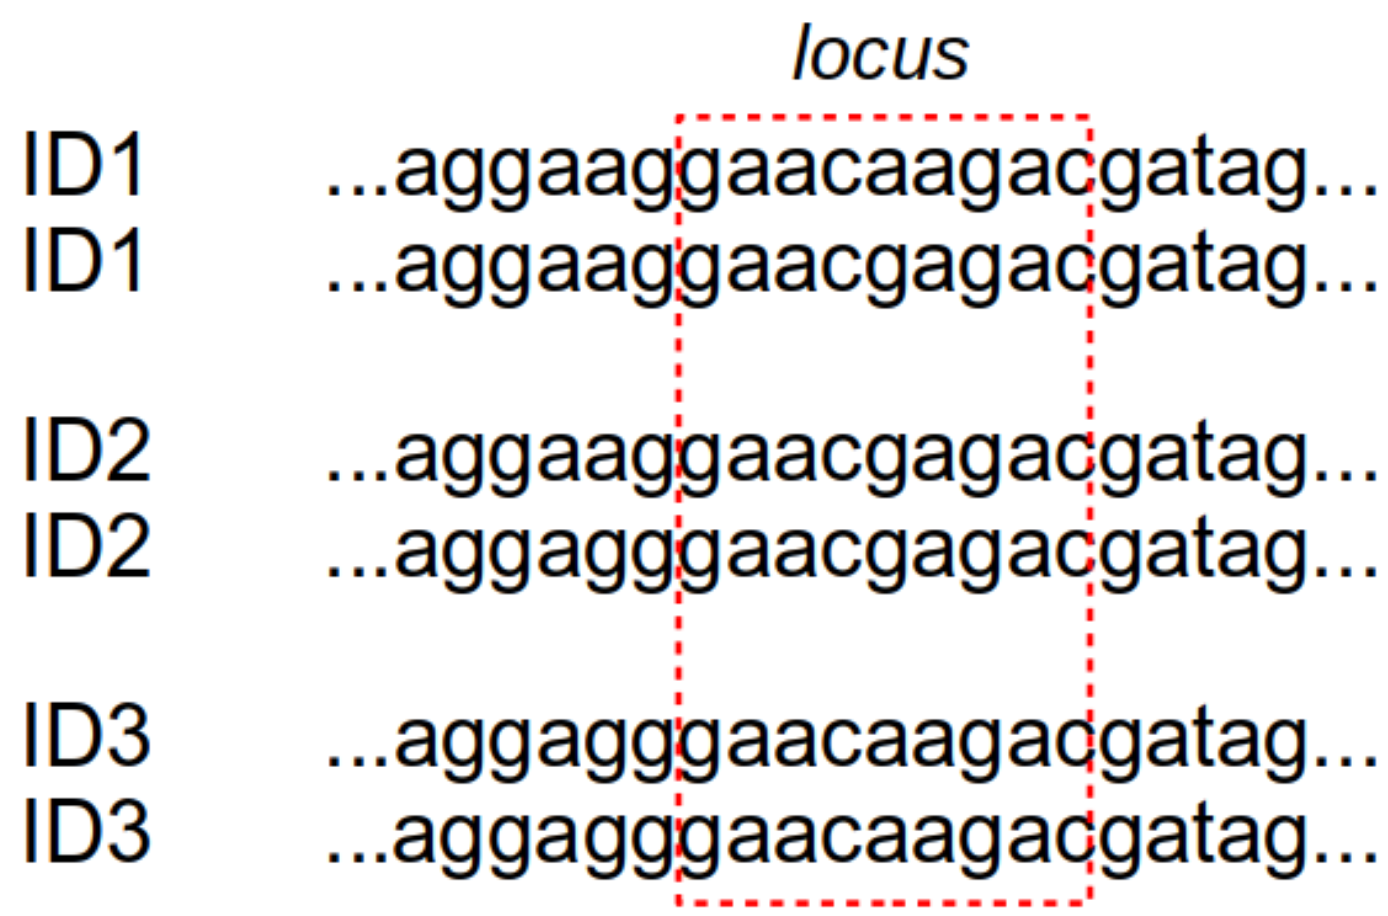
\includegraphics[width=.6\textwidth]{graphics_day2a_popgen/locus_example.png}\\[2ex]
		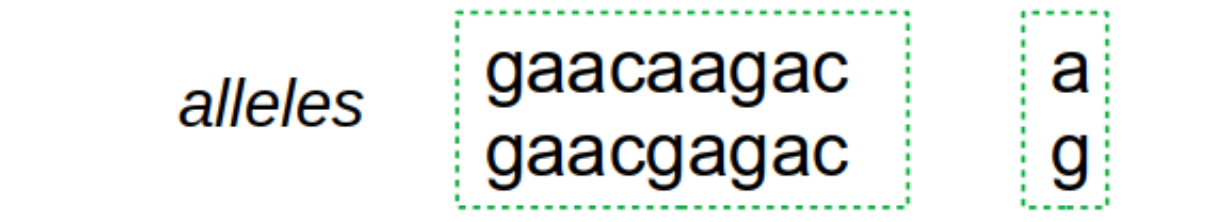
\includegraphics[width=.6\textwidth]{graphics_day2a_popgen/allele_example.png}
	\end{center}
	\caption{A \emph{locus} of nine base pairs (bp) and two alleles.}
	\end{figure}
\end{frame}
%%%%%%%%%%%%%%%%%%%%%%%%%%%%%%%%%%%%%%%%%%%%%%%%%%%%%%%%%%%%%%%%%%%%%%%%%%%%%%%%%%%%%%
%
%
%
%%%%%%%%%%%%%%%%%%%%%%%%%%%%%%%%%%%%%%%%%%%%%%%%%%%%%%%%%%%%%%%%%%%%%%%%%%%%%%%%%%%%%%
\begin{frame}\frametitle{Genotype}
	A \textbf{genotype} can be defined as the genetic makeup of an individual (at one or more loci).\\[2ex]
	It can also be considered as a description of the alleles possessed by an individual.
\end{frame}
%%%%%%%%%%%%%%%%%%%%%%%%%%%%%%%%%%%%%%%%%%%%%%%%%%%%%%%%%%%%%%%%%%%%%%%%%%%%%%%%%%%%%%
%
%
%
%%%%%%%%%%%%%%%%%%%%%%%%%%%%%%%%%%%%%%%%%%%%%%%%%%%%%%%%%%%%%%%%%%%%%%%%%%%%%%%%%%%%%%
\begin{frame}\frametitle{Genotype}
	\begin{figure}
	\begin{center}
		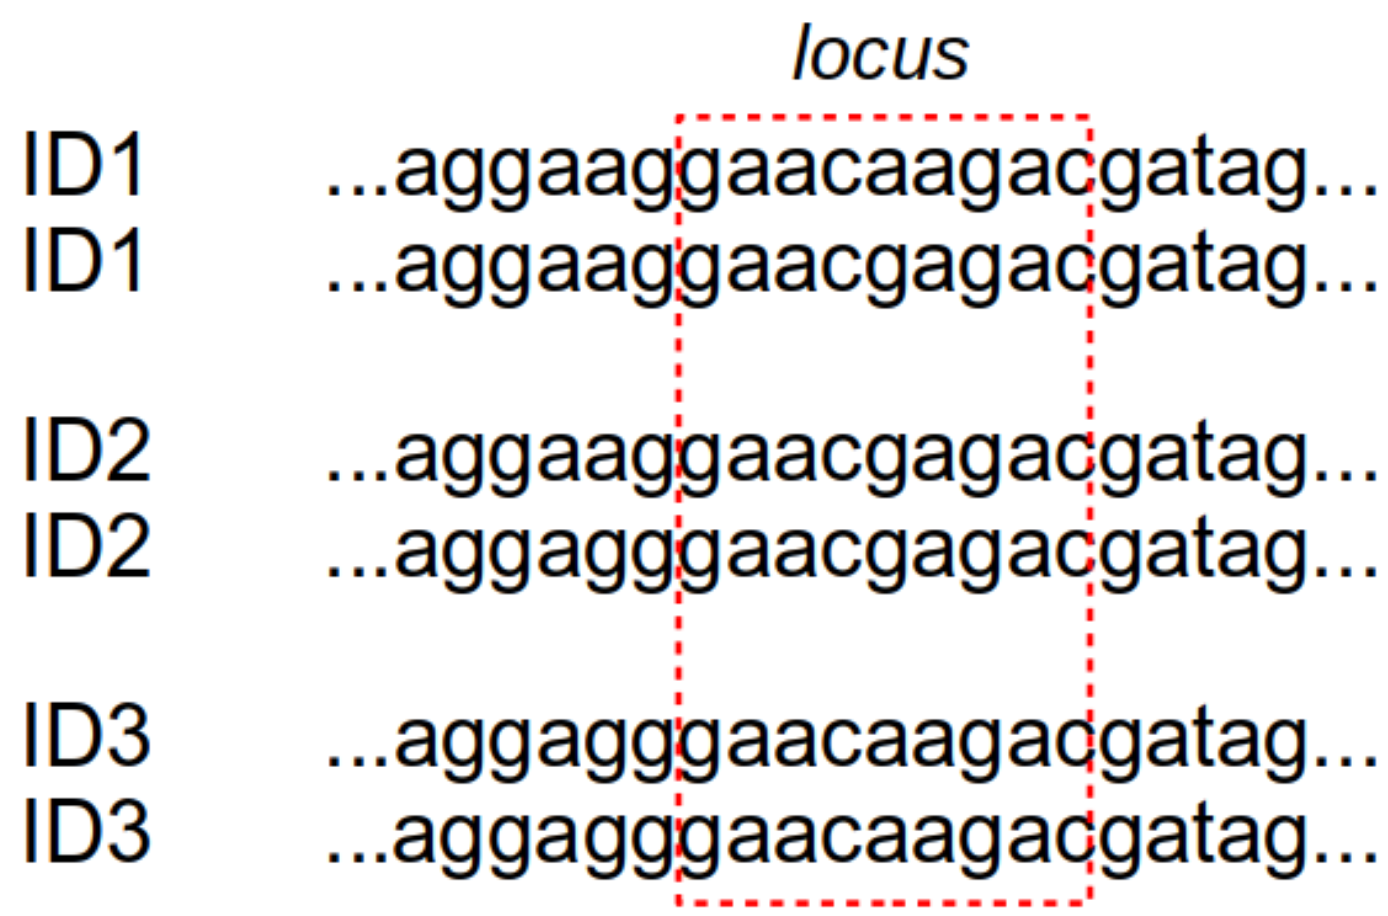
\includegraphics[width=.6\textwidth]{graphics_day2a_popgen/locus_example.png}
		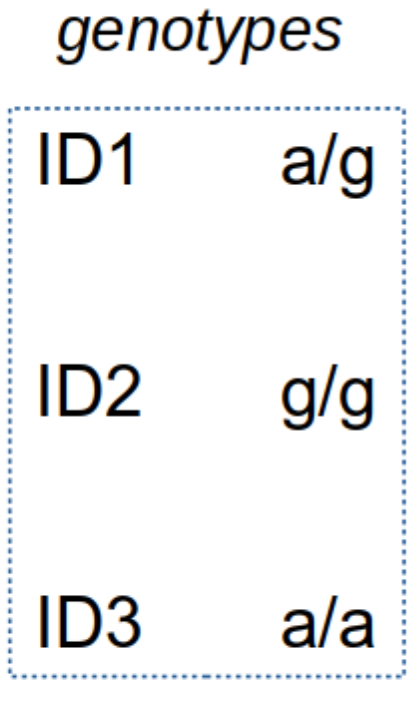
\includegraphics[width=.225\textwidth]{graphics_day2a_popgen/genotypes_example.png}\\[2ex]
		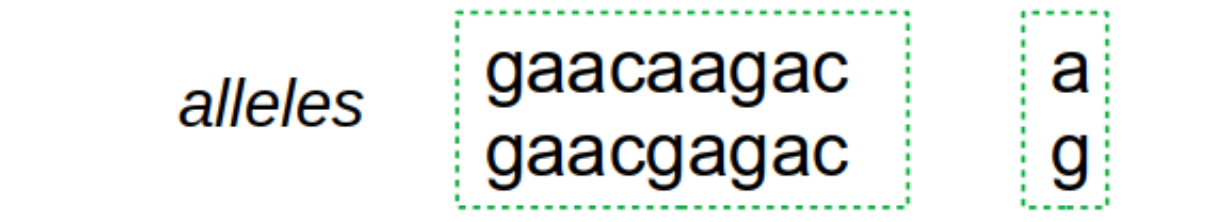
\includegraphics[width=.6\textwidth]{graphics_day2a_popgen/allele_example.png}\phantom{menace}\phantom{menace}
	\end{center}
	\caption{A \emph{locus} of nine base pairs (bp), two alleles, and three genotypes.}
	\end{figure}
\end{frame}
%%%%%%%%%%%%%%%%%%%%%%%%%%%%%%%%%%%%%%%%%%%%%%%%%%%%%%%%%%%%%%%%%%%%%%%%%%%%%%%%%%%%%%
%
%
%
%%%%%%%%%%%%%%%%%%%%%%%%%%%%%%%%%%%%%%%%%%%%%%%%%%%%%%%%%%%%%%%%%%%%%%%%%%%%%%%%%%%%%%
\begin{frame}\frametitle{Haplotype}
	A \textbf{haplotype}$^{*}$ is the series of alleles along the same chromosome.
	\begin{figure}
	\begin{center}
		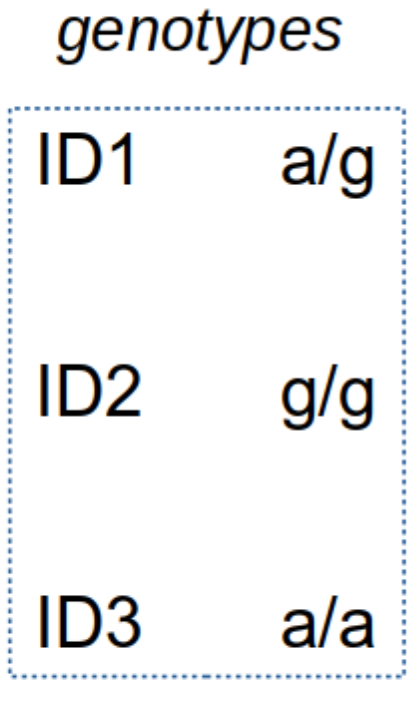
\includegraphics[width=.215\textwidth]{graphics_day2a_popgen/genotypes_example.png}
		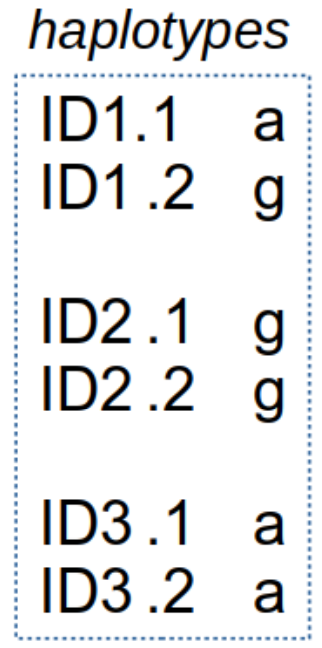
\includegraphics[width=.19\textwidth]{graphics_day2a_popgen/haplotypes_example.png}
	\end{center}
	\caption{Difference between genotype and haplotype.}
	\end{figure}
	{\tiny $^{*}$In the literature there are discordant definitions and you will sometimes find terms alleles and haplotypes being used interchangeably. In some textbooks you may find that haplotypes refer to chromosomes while allotypes refer to what we define here as haplotypes.}
\end{frame}
%%%%%%%%%%%%%%%%%%%%%%%%%%%%%%%%%%%%%%%%%%%%%%%%%%%%%%%%%%%%%%%%%%%%%%%%%%%%%%%%%%%%%%
%
%
%
%%%%%%%%%%%%%%%%%%%%%%%%%%%%%%%%%%%%%%%%%%%%%%%%%%%%%%%%%%%%%%%%%%%%%%%%%%%%%%%%%%%%%%
\begin{frame}\frametitle{Diploids}
	What happens if you have multiple copies of each chromosome?\\[2ex]
	As \emph{diploid} species have two copies of their chromosomes, for a collection of $N$ diploid individuals, there are $2N$ gene copies at each locus, with one or more alleles.\\[2ex]
	As mutations are rare in most organisms, \textbf{bi-allelic} models are often used, with at most two alleles at each locus$^{*}$.\\[2ex]
	{\small $^{*}$E.g., at the red-hair vs. non-red-hair locus in \emph{MC1R}, most individuals have \texttt{C}, some have \texttt{T}, but \texttt{A} and \texttt{G} have not been observed suggesting a bi-allelic model is a valid approximation here.}
\end{frame}
%%%%%%%%%%%%%%%%%%%%%%%%%%%%%%%%%%%%%%%%%%%%%%%%%%%%%%%%%%%%%%%%%%%%%%%%%%%%%%%%%%%%%%
%
%
%
%%%%%%%%%%%%%%%%%%%%%%%%%%%%%%%%%%%%%%%%%%%%%%%%%%%%%%%%%%%%%%%%%%%%%%%%%%%%%%%%%%%%%%
\begin{frame}\frametitle{Terminology}
	Before we dive into the genetic basis of evolution, let us define some important terms, such as:
	\begin{itemize}
		\item Gene
		\item Phenotype
		\item Locus
		\item Allele
		\item Genotype
		\item Haplotype
	\end{itemize}
\end{frame}
%%%%%%%%%%%%%%%%%%%%%%%%%%%%%%%%%%%%%%%%%%%%%%%%%%%%%%%%%%%%%%%%%%%%%%%%%%%%%%%%%%%%%%
%
%
%
%%%%%%%%%%%%%%%%%%%%%%%%%%%%%%%%%%%%%%%%%%%%%%%%%%%%%%%%%%%%%%%%%%%%%%%%%%%%%%%%%%%%%%
\begin{frame}\frametitle{Evolutionary genetics}
	Now that all the main terminology has been defined, we can have a closer look at the genetics of evolution.
	\begin{block}{What is evolutionary genetics?}
		In evolutionary genetics we are interested in studying the genetic \textbf{variation} between/within species/populations. It is both:
		\begin{itemize}
			\item \textbf{Retrospective}: Understanding what determined the current genetic composition of a species/population.
			\item \textbf{Predictive}: Predicting the future composition of a species/population from its current composition.
		\end{itemize}
	\end{block}
\end{frame}
%%%%%%%%%%%%%%%%%%%%%%%%%%%%%%%%%%%%%%%%%%%%%%%%%%%%%%%%%%%%%%%%%%%%%%%%%%%%%%%%%%%%%%
%
%
%
%%%%%%%%%%%%%%%%%%%%%%%%%%%%%%%%%%%%%%%%%%%%%%%%%%%%%%%%%%%%%%%%%%%%%%%%%%%%%%%%%%%%%%
\begin{frame}\frametitle{Evolution}
	\begin{block}{How do we ``measure'' evolution?}
		The simplest definition of evolution is ``a change in allele frequencies over time''.
	\end{block}
	Therefore, we first need to understand how changes in allele frequencies occur.\\[2ex]
	But before that, what is an \textbf{allele frequency}? How do we calculate them? Is there a concept of \textbf{genotype frequency}?
\end{frame}
%%%%%%%%%%%%%%%%%%%%%%%%%%%%%%%%%%%%%%%%%%%%%%%%%%%%%%%%%%%%%%%%%%%%%%%%%%%%%%%%%%%%%%
%
%
%
%%%%%%%%%%%%%%%%%%%%%%%%%%%%%%%%%%%%%%%%%%%%%%%%%%%%%%%%%%%%%%%%%%%%%%%%%%%%%%%%%%%%%%
\begin{frame}\frametitle{Allele and genotype frequency}
\only<1-8>{Assume that we have a population of $N = 10$ diploid individuals (thus $2N = 20$ gene copies), and a total of 7 copies of allele $A$ (yellow) and 13 copies of allele $a$ (blue).}
	\begin{columns}
	\begin{column}{.36\textwidth}
		\begin{center}
		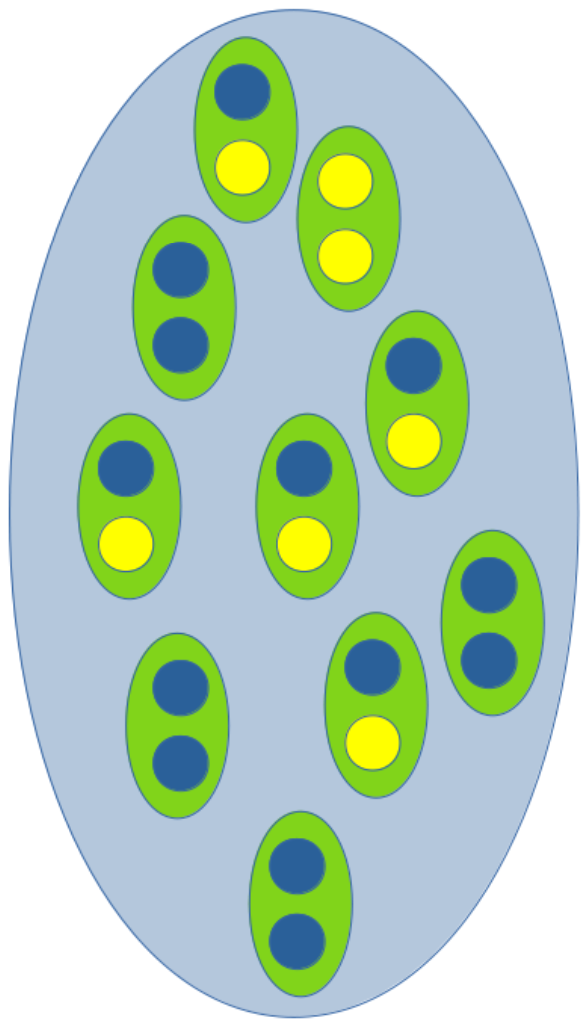
\includegraphics[width=.7\textwidth]{graphics_day2a_popgen/alleles_in_population.png}
		\end{center}
	\end{column}
	\begin{column}{.64\textwidth}
\only<1>{%
		What are the allele frequencies?\\[2ex]
		How would you calculate, for example, $f_A$, the frequency of alleles $A$ (yellow) within this population?\\[1ex]
		Try to find the answer yourself before moving to the next slide. $f_A =$?
}
\only<2>{%
		\vspace{0ex}\\What are the allele frequencies?\\[2ex]
		$f_A = 7/20 = 0.35$,\\
		because we have 7 $A$ alleles out of 20 in total.\\
		How about $f_a$, the frequency of allele $a$ (blue)?\\[2ex]
		Try to find the answer yourself before moving to the next slide. $f_a =$?
}
\only<3-4>{%
		\vspace{1ex}\\What are the allele frequencies?\\[2ex]
		$f_A = 7/20 = 0.35$\\
		$f_a = 13/20 = 0.65$,\\
		because we have 13 a alleles out of 20 in total.\\[2ex]
		Do you notice a relationship between $f_A$ and $f_a$? \visible<4>{Their sum is 1! $0.35 + 0.65 = 1$, and this is a true general statement: $f_A + f_a = 1$ for bi-allelic variation.}
}
\only<5>{%
		\vspace{1ex}\\What are the \textbf{allele} frequencies?\\[1.5ex]
		$f_A = 7/20 = 0.35$\\
		$f_a = 13/20 = 0.65$\\[1.5ex]
		What are the \textbf{genotype} frequencies? Before answering this question, what are the genotypes in this example? You have diploid individuals with two possible alleles $A $(yellow) and $a$ (blue).\\[1.5ex]
		Try to find the answer yourself before moving to the next slide.
}
\only<6>{%
		\vspace{1ex}\\What are the \textbf{allele} frequencies?\\[1.5ex]
		$f_A = 7/20 = 0.35$\\
		$f_a = 13/20 = 0.65$\\[1.5ex]
		What are the \textbf{genotype} frequencies?\\[1.5ex]
		We have three possible genotypes: \{$AA$, $Aa$, $aa$\} or \{yellow/yellow, yellow/blue, blue/blue\}.\\[1.5ex]
		What are their frequencies? Count them and check the answer on the next slide.
}
\only<7-8>{%
		\vspace{1ex}\\What are the allele and genotype frequencies?\\[1.5ex]
		$f_A = 7/20$\\
		$f_a = 13/20$\\[1.5ex]
		$f_{AA} =$\visible<8>{$\:1/10$\\
		$f_{Aa} = 5/10$\\
		$f_{aa} = 4/10$\\[1.5ex]
		We say that $AA$ and $aa$ are \textbf{homozygous} individuals and $Aa$ are \textbf{heterozygous} individuals.\\
		Note again that $f_{AA} + f_{Aa} + f_{aa} = 1$.}
}
\only<9>{%
		\vspace{0ex}\\The proportion of heterozygous individuals in the population ($f_{Aa}$) is called the \textbf{heterozygosity}.\\[2ex]
		The proportion of homozygotes ($1 - f_{Aa} = f_{AA} + f_{aa}$) is the \textbf{homozygosity} of the population.
}
	\end{column}
	\end{columns}
\end{frame}
%%%%%%%%%%%%%%%%%%%%%%%%%%%%%%%%%%%%%%%%%%%%%%%%%%%%%%%%%%%%%%%%%%%%%%%%%%%%%%%%%%%%%%
%
%
%
%%%%%%%%%%%%%%%%%%%%%%%%%%%%%%%%%%%%%%%%%%%%%%%%%%%%%%%%%%%%%%%%%%%%%%%%%%%%%%%%%%%%%%
\begin{frame}\frametitle{MC1R gene}
	Here is a challenge for you. The SNPs coded as rs1805007 in the human \emph{MC1R} gene is associated with red hair$^{*}$.
	\begin{figure}
	\begin{center}
		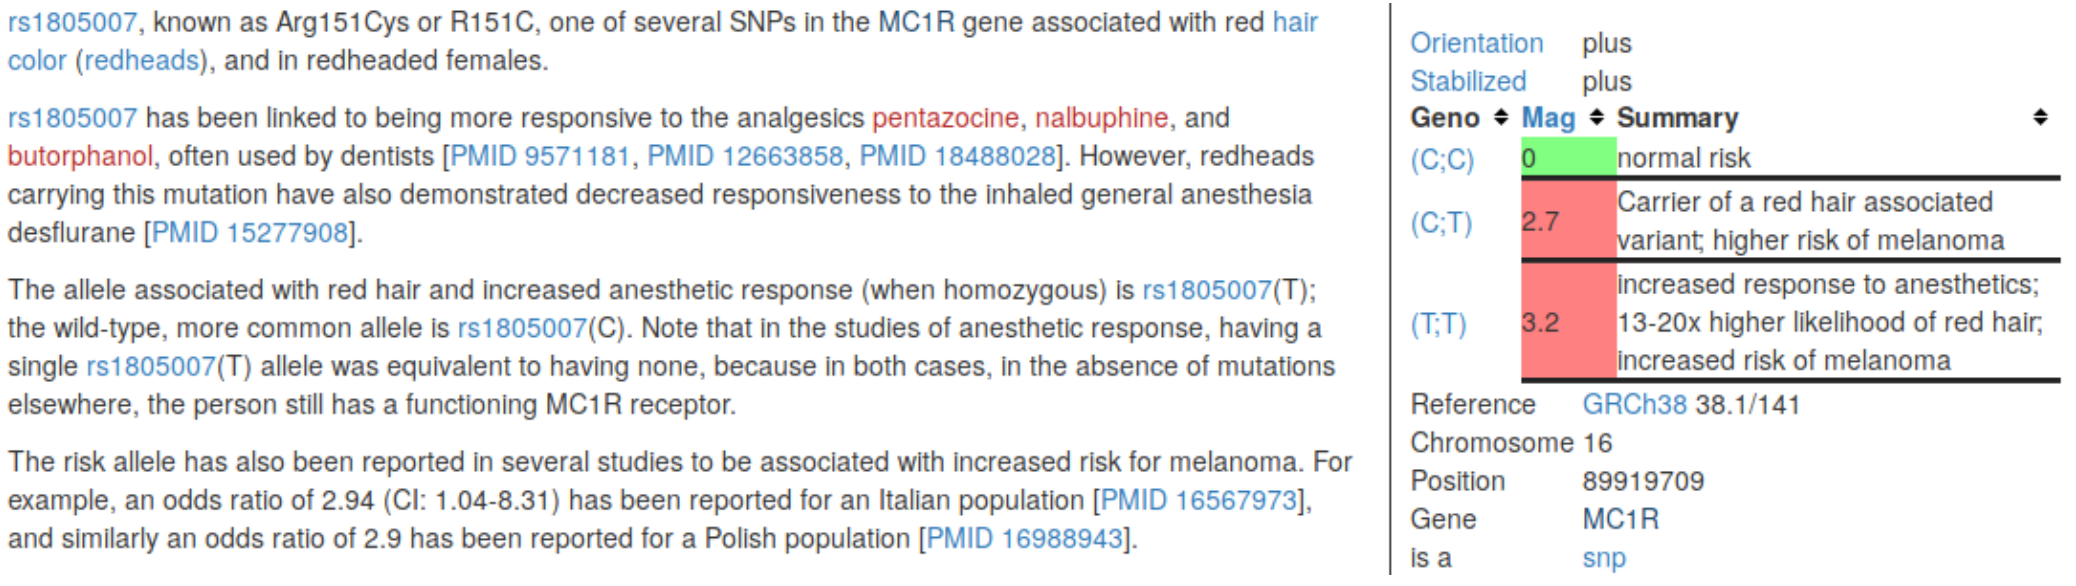
\includegraphics[width=\textwidth]{graphics_day2a_popgen/mc1r_snp.png}
	\end{center}
	\caption{SNP associated to red hair with alleles \texttt{C} and \texttt{T}.}
	\end{figure}
	{\tiny $^{*}$\url{https://www.snpedia.com/index.php/Rs1805007}}
\end{frame}
%%%%%%%%%%%%%%%%%%%%%%%%%%%%%%%%%%%%%%%%%%%%%%%%%%%%%%%%%%%%%%%%%%%%%%%%%%%%%%%%%%%%%%
%
%
%
%%%%%%%%%%%%%%%%%%%%%%%%%%%%%%%%%%%%%%%%%%%%%%%%%%%%%%%%%%%%%%%%%%%%%%%%%%%%%%%%%%%%%%
\begin{frame}\frametitle{MC1R gene}
	Assume we obtain a \emph{random} sample of 30 individuals from the population in the UK and find that 25 individuals have genotype \texttt{CC}, 5 individuals have genotype \texttt{CT} and 0 have genotype \texttt{TT} at SNP rs1805007.
	\begin{enumerate}
		\item What are the estimated genotype frequencies?
		\item What are the estimated homozygosity and heterozygosity in the population?
		\item What are the estimated allele frequencies? How do you calculate them?
		\item Why are these frequencies estimated and not calculated?
	\end{enumerate}
\end{frame}
%%%%%%%%%%%%%%%%%%%%%%%%%%%%%%%%%%%%%%%%%%%%%%%%%%%%%%%%%%%%%%%%%%%%%%%%%%%%%%%%%%%%%%
%
%
%
%%%%%%%%%%%%%%%%%%%%%%%%%%%%%%%%%%%%%%%%%%%%%%%%%%%%%%%%%%%%%%%%%%%%%%%%%%%%%%%%%%%%%%
\begin{frame}\frametitle{Allele frequencies in time}
	\begin{columns}
	\begin{column}{.36\textwidth}
		\begin{center}
		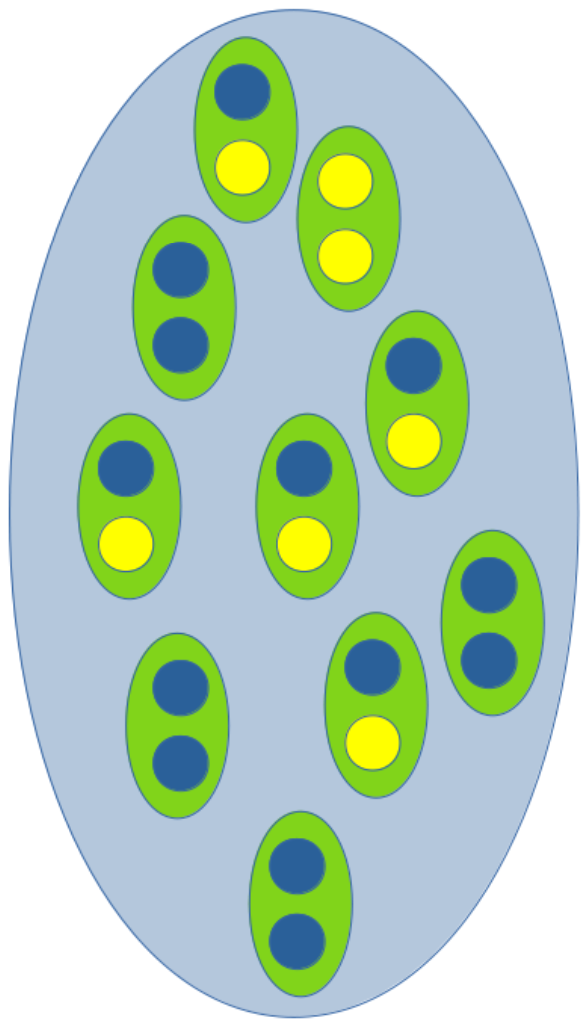
\includegraphics[width=.7\textwidth]{graphics_day2a_popgen/alleles_in_population.png}
		\end{center}
	\end{column}
	\begin{column}{.64\textwidth}
		\begin{block}{}
			We focus on describing the changes of $f_A$ and $f_a$ with time.
		\end{block}\vspace{2ex}
		If we can describe how we expect allele frequencies to change through time in a population, we have gained important insights into its evolution.
	\end{column}
	\end{columns}
\end{frame}
%%%%%%%%%%%%%%%%%%%%%%%%%%%%%%%%%%%%%%%%%%%%%%%%%%%%%%%%%%%%%%%%%%%%%%%%%%%%%%%%%%%%%%
%
%
%
%%%%%%%%%%%%%%%%%%%%%%%%%%%%%%%%%%%%%%%%%%%%%%%%%%%%%%%%%%%%%%%%%%%%%%%%%%%%%%%%%%%%%%
\begin{frame}\frametitle{Alleles to genotypes}
	We can calculate allele frequencies from genotype frequencies.
	\begin{block}{}
		Can we \emph{predict} genotype frequencies from allele frequencies?
	\end{block}
	For example, if we know that the frequency of allele \texttt{T} at position 478 of the human gene \emph{MC1R} is 0.08, what proportion of the population is expected to have genotype \texttt{TT}?
\end{frame}
%%%%%%%%%%%%%%%%%%%%%%%%%%%%%%%%%%%%%%%%%%%%%%%%%%%%%%%%%%%%%%%%%%%%%%%%%%%%%%%%%%%%%%
%
%
%
%%%%%%%%%%%%%%%%%%%%%%%%%%%%%%%%%%%%%%%%%%%%%%%%%%%%%%%%%%%%%%%%%%%%%%%%%%%%%%%%%%%%%%
\begin{frame}
	Can we \emph{predict} genotype frequencies from allele frequencies?\\
	Can we go back and forth between these two figures (genotypes on the left hand side and alleles on the right hand side)?
	\begin{center}
		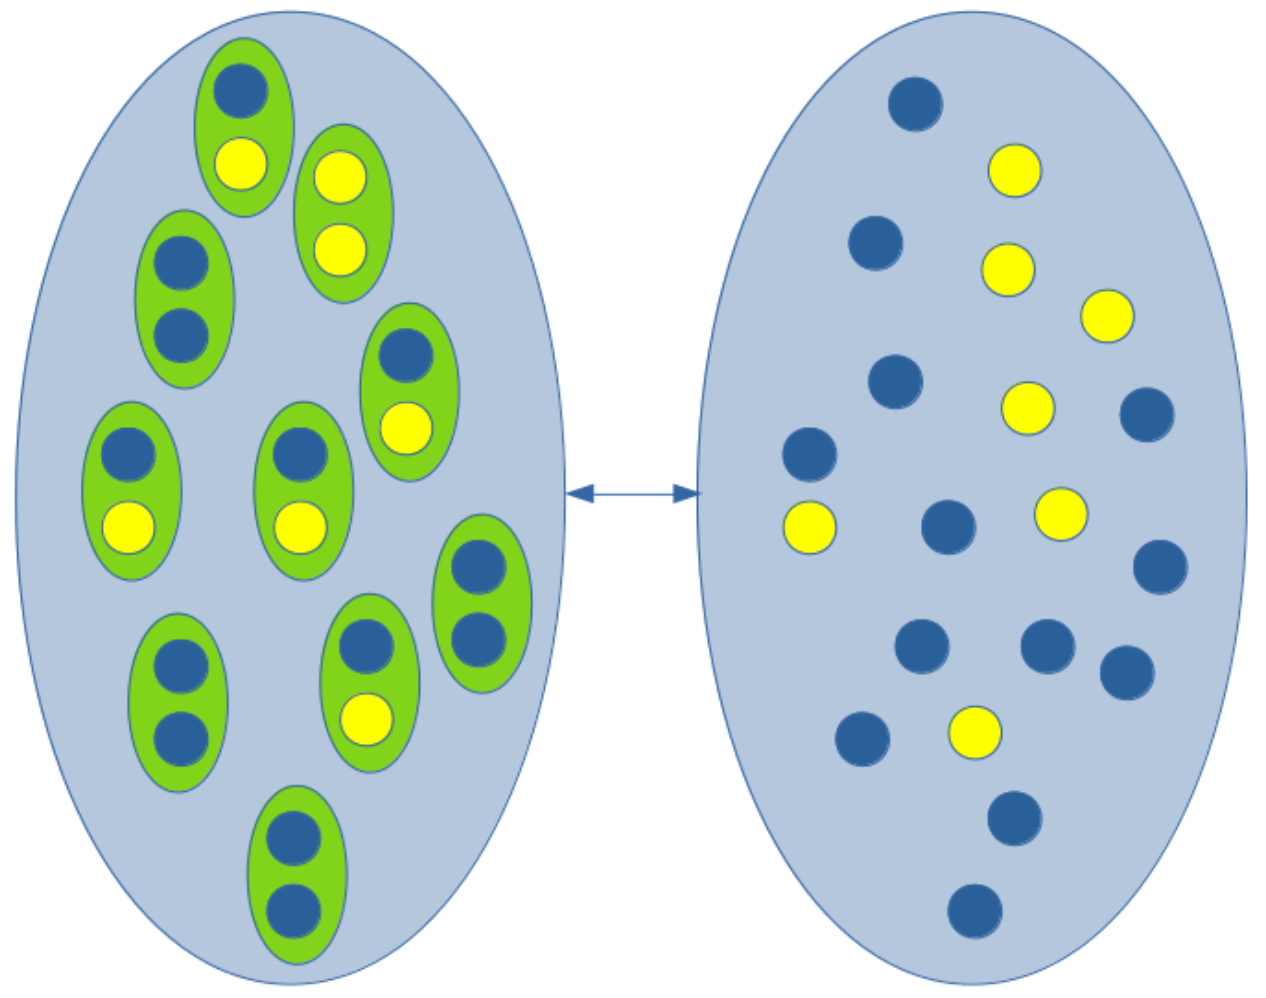
\includegraphics[width=.6\textwidth]{graphics_day2a_popgen/allele_freq_to_geno.png}
	\end{center}
\end{frame}
%%%%%%%%%%%%%%%%%%%%%%%%%%%%%%%%%%%%%%%%%%%%%%%%%%%%%%%%%%%%%%%%%%%%%%%%%%%%%%%%%%%%%%
%
%
%
%%%%%%%%%%%%%%%%%%%%%%%%%%%%%%%%%%%%%%%%%%%%%%%%%%%%%%%%%%%%%%%%%%%%%%%%%%%%%%%%%%%%%%
\begin{frame}
	Can we \emph{predict} genotype frequencies from allele frequencies?\\
	Yes, under these assumptions:
	\begin{itemize}
		\item The organism is diploid.
		\item The locus is bi-allelic.
		\item Reproduction is sexual.
		\item Generations are non-overlapping.
		\item Mating is random: Individuals mate with each other without regard to their genotype.
		\item Populations are ``infinite'' (very large in size).
		\item There is no mutation, migration, natural selection or drift$^{*}$.
	\end{itemize}
	If these conditions are met, we can calculate genotype frequencies under \textbf{Hardy-Weinberg Equilibrium (HWE)}.\\[1.5ex]
	{\scriptsize $^{*}$We will learn what these terms mean later on.}
\end{frame}
%%%%%%%%%%%%%%%%%%%%%%%%%%%%%%%%%%%%%%%%%%%%%%%%%%%%%%%%%%%%%%%%%%%%%%%%%%%%%%%%%%%%%%
%
%
%
%%%%%%%%%%%%%%%%%%%%%%%%%%%%%%%%%%%%%%%%%%%%%%%%%%%%%%%%%%%%%%%%%%%%%%%%%%%%%%%%%%%%%%
\begin{frame}\frametitle{Hardy-Weinberg Equilibrium (HWE)}
	From the allele frequencies $f_A$ and $f_a$ we can calculate the \emph{expected} genotype frequencies under HWE as follows:
	\begin{center}
	\setlength{\tabcolsep}{12pt}
	\begin{tabular}{llll}
		\toprule
		\multicolumn{4}{l}{Genotype frequencies under HWE} \\
		\midrule
		Genotype	& $AA$		& $Aa$			& $aa$		\\
		Frequency	& $f_A^2$	& $2f_A f_a$	& $f_a^2$	\\
		\bottomrule
	\end{tabular}
	\setlength{\tabcolsep}{6pt}
	\end{center}
\end{frame}
%%%%%%%%%%%%%%%%%%%%%%%%%%%%%%%%%%%%%%%%%%%%%%%%%%%%%%%%%%%%%%%%%%%%%%%%%%%%%%%%%%%%%%
%
%
%
%%%%%%%%%%%%%%%%%%%%%%%%%%%%%%%%%%%%%%%%%%%%%%%%%%%%%%%%%%%%%%%%%%%%%%%%%%%%%%%%%%%%%%
\begin{frame}\frametitle{Hardy-Weinberg Equilibrium (HWE)}
	From the HWE equations we learn that:\\[2ex]
	\begin{enumerate}
		\item $f_A^2 + 2f_A f_a + f_a^2 = 1$
		\item Random mating does not change the allele frequencies in the next generation.
	\end{enumerate}\vspace{2ex}
	In other words, under HWE we do not expect to see \emph{on average} a change in allele frequency from one generation to the next.
\end{frame}
%%%%%%%%%%%%%%%%%%%%%%%%%%%%%%%%%%%%%%%%%%%%%%%%%%%%%%%%%%%%%%%%%%%%%%%%%%%%%%%%%%%%%%
%
%
%
%%%%%%%%%%%%%%%%%%%%%%%%%%%%%%%%%%%%%%%%%%%%%%%%%%%%%%%%%%%%%%%%%%%%%%%%%%%%%%%%%%%%%%
\begin{frame}\frametitle{HWE in \emph{MC1R}}
	\begin{columns}
	\begin{column}{.5\textwidth}
		\begin{figure}
		\begin{center}
			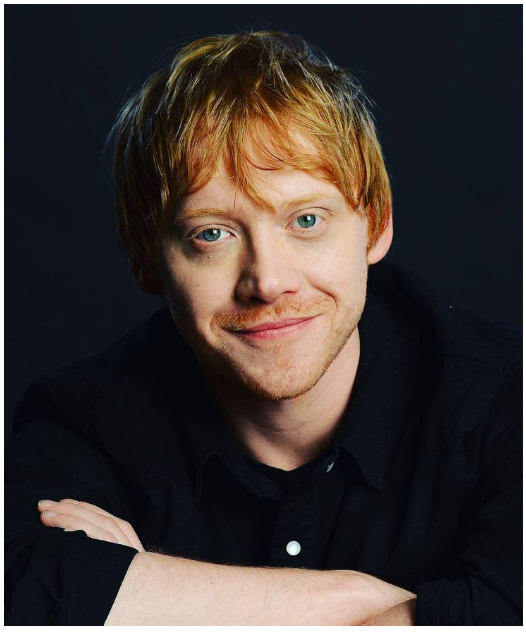
\includegraphics[width=.5\textwidth]{graphics_day2a_popgen/rupert_grint.png}
		\end{center}
		\caption{Rupert Grint.}
		\end{figure}
	\end{column}
	\begin{column}{.5\textwidth}
		With an allele frequency of 0.08 for allele \texttt{T} in the UK population, how many \texttt{TT} homozygotes might we expect under HWE?\\
		\visible<2>{It’s $0.08^2 = 0.0064$.\\[2ex]
		Individuals with \texttt{TT} genotype will likely have red hair, but a much larger proportion of the population has red hair.}
	\end{column}
	\end{columns}
\end{frame}
%%%%%%%%%%%%%%%%%%%%%%%%%%%%%%%%%%%%%%%%%%%%%%%%%%%%%%%%%%%%%%%%%%%%%%%%%%%%%%%%%%%%%%
%
%
%
%%%%%%%%%%%%%%%%%%%%%%%%%%%%%%%%%%%%%%%%%%%%%%%%%%%%%%%%%%%%%%%%%%%%%%%%%%%%%%%%%%%%%%
\begin{frame}\frametitle{Deviations from HWE}
	\begin{itemize}
		\item Assortative mating: Not random with respect to genotype.
		\item Inbreeding: Mating of related individuals.
		\item Population structure: Sample of individuals from two or more subpopulations.
		\item Natural selection: Alleles affect the \emph{fitness}$^{*}$ of the carrier.
	\end{itemize}
	\vspace{1ex}{\small $^{*}$More on this later.}
\end{frame}
%%%%%%%%%%%%%%%%%%%%%%%%%%%%%%%%%%%%%%%%%%%%%%%%%%%%%%%%%%%%%%%%%%%%%%%%%%%%%%%%%%%%%%
%
%
%
%%%%%%%%%%%%%%%%%%%%%%%%%%%%%%%%%%%%%%%%%%%%%%%%%%%%%%%%%%%%%%%%%%%%%%%%%%%%%%%%%%%%%%
\begin{frame}\frametitle{Inbreeding coefficient}
	\begin{block}{Inbreeding coefficient ($F$)}
		Most common statistic to measure deviations from HWE: It describes the degree to which heterozygosity is reduced both in individuals and in populations.
	\end{block}
	\begin{equation}
		F = \frac{2f_A f_a - f_{Aa}}{2f_A f_a}
	\end{equation}
	$~$\\[-0.5ex]If $F = 0$, the population is in HWE. If $F = 1$, \visible<2>{there are no heterozygotes.}
\end{frame}
%%%%%%%%%%%%%%%%%%%%%%%%%%%%%%%%%%%%%%%%%%%%%%%%%%%%%%%%%%%%%%%%%%%%%%%%%%%%%%%%%%%%%%
%
%
%
%%%%%%%%%%%%%%%%%%%%%%%%%%%%%%%%%%%%%%%%%%%%%%%%%%%%%%%%%%%%%%%%%%%%%%%%%%%%%%%%%%%%%%
\begin{frame}\frametitle{Inbreeding coefficient}
	\begin{equation}
		f_{Aa} = 2 f_A f_a (1 - F)
	\end{equation}
	\begin{itemize}
		\item The proportion of heterozygotes in the population is reduced by a factor of F from that expected under HWE.
		\item If we know F and the allele frequencies, we can predict genotype frequencies without assuming HWE.
	\end{itemize}
	Are there species likely to deviate from HWE?
\end{frame}
%%%%%%%%%%%%%%%%%%%%%%%%%%%%%%%%%%%%%%%%%%%%%%%%%%%%%%%%%%%%%%%%%%%%%%%%%%%%%%%%%%%%%%
%
%
%
%%%%%%%%%%%%%%%%%%%%%%%%%%%%%%%%%%%%%%%%%%%%%%%%%%%%%%%%%%%%%%%%%%%%%%%%%%%%%%%%%%%%%%
\begin{frame}\frametitle{Self-fertilizing plants}
	\begin{columns}
	\begin{column}{.45\textwidth}
		\begin{figure}
		\begin{center}
			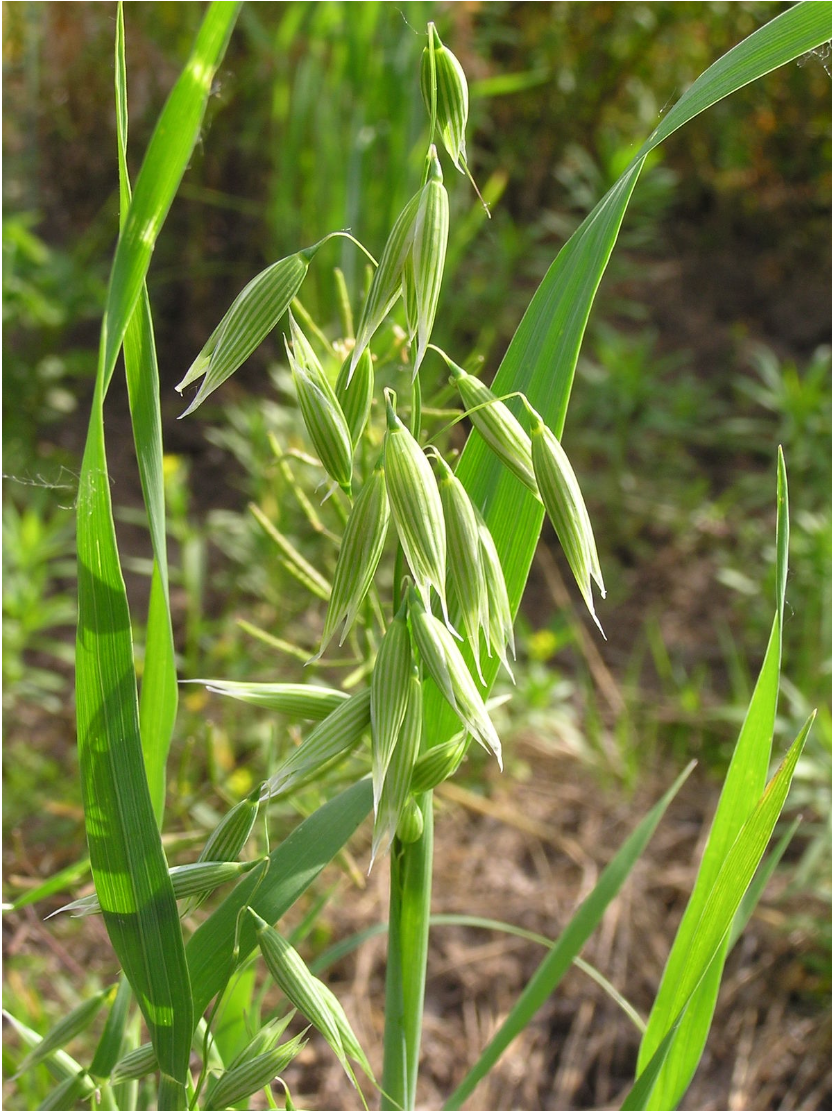
\includegraphics[width=.9\textwidth]{graphics_day2a_popgen/avena_fatua.png}
		\end{center}
		\caption{Flower of wild oats (Avena fatua).}
		\end{figure}
	\end{column}
	\begin{column}{.55\textwidth}
		Genotype frequencies at one locus are:\\
		$f_{AA} = 0.58, f_{Aa} = 0.07, f_{aa} = 0.35$.
		\begin{enumerate}
			\item What is F, the inbreeding coefficient?\\
\visible<2>{{\small $f_A = 0.58 + 0.07/2 = 0.615$,\\
				$f_a = 1-0.615 = 0.385$,\\
				$2f_A f_a = 2\times0.385\times0.615 = 0.474$,\\
				$F = (0.474-0.07)/0.474 = 0.852$.}
			\item Does it deviate from HWE?
}
		\end{enumerate}
	\end{column}
	\end{columns}
\end{frame}
%%%%%%%%%%%%%%%%%%%%%%%%%%%%%%%%%%%%%%%%%%%%%%%%%%%%%%%%%%%%%%%%%%%%%%%%%%%%%%%%%%%%%%
%
%
%
%%%%%%%%%%%%%%%%%%%%%%%%%%%%%%%%%%%%%%%%%%%%%%%%%%%%%%%%%%%%%%%%%%%%%%%%%%%%%%%%%%%%%%
\begin{frame}\frametitle{Testing for deviations from HWE}
	\begin{columns}
	\begin{column}{.3\textwidth}
		\begin{center}
		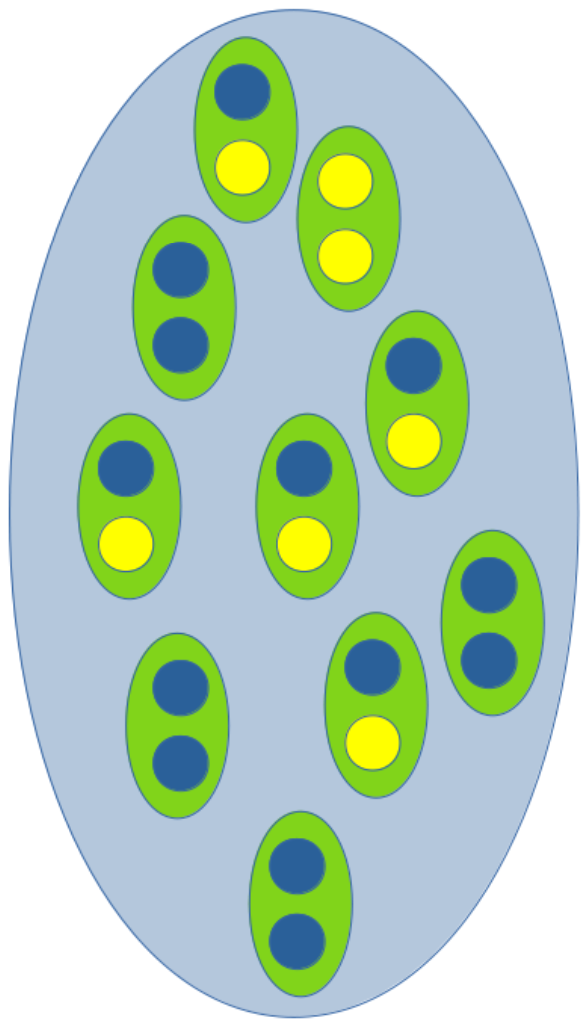
\includegraphics[width=.8\textwidth]{graphics_day2a_popgen/alleles_in_population.png}
		\end{center}
	\end{column}
	\begin{column}{.7\textwidth}
		\begin{itemize}
			\item A random sample for a population in HWE may deviate from HWE.
			\item We need a formal statistical test:\\[1.5ex]
				\underline{Null hypothesis:} Genotype frequencies follow those predicted by HWE.\\[1.5ex]
				\underline{Alternative hypothesis:} genotype frequencies do \textbf{not} follow those predicted by HWE
		\end{itemize}
	\end{column}
	\end{columns}
\end{frame}
%%%%%%%%%%%%%%%%%%%%%%%%%%%%%%%%%%%%%%%%%%%%%%%%%%%%%%%%%%%%%%%%%%%%%%%%%%%%%%%%%%%%%%
%
%
%
%%%%%%%%%%%%%%%%%%%%%%%%%%%%%%%%%%%%%%%%%%%%%%%%%%%%%%%%%%%%%%%%%%%%%%%%%%%%%%%%%%%%%%
\begin{frame}\frametitle{Testing for deviations from HWE}
	Chi-square test: $\chi^2 = \sum_{i=1}^k \frac{(E_i - O_i)^2}{E_i}$
	\begin{itemize}
		\item Observed values $O_i$ (genotype counts).
		\item Expected values $E_i$ (expected genotype counts under HWE).
		\item Degrees of freedom: $3-1-1=1$.
	\end{itemize}
	If $\chi^2$ is large enough, we reject the null hypothesis.
\end{frame}
%%%%%%%%%%%%%%%%%%%%%%%%%%%%%%%%%%%%%%%%%%%%%%%%%%%%%%%%%%%%%%%%%%%%%%%%%%%%%%%%%%%%%%
%
%
%
%%%%%%%%%%%%%%%%%%%%%%%%%%%%%%%%%%%%%%%%%%%%%%%%%%%%%%%%%%%%%%%%%%%%%%%%%%%%%%%%%%%%%%
\begin{frame}\frametitle{Testing for deviations from HWE}
	$\chi^2 = \sum_{i=1}^k \frac{(E_i - O_i)^2}{E_i}$\\[1.5ex]
	Observed genotype counts: $O_{AA} = 20$, $O_{Aa} = 10$, $O_{aa} = 10$.
	\begin{itemize}
\visible<2->{\item $f_{AA} =1/2$, $f_{Aa} =1/4$, $f_{aa} =1/4$.}
\visible<3->{\item $f_A =1/2+(1/4)/2=5/8$, $f_a =1/4+(1/4)/2=3/8$.}
\visible<4->{\item $E_{AA} =40\times(5/8)^2 =15.625$, $E_{Aa} =40\times2\times3/8\times5/8=18.75$, $E_{aa} = 40 \times (3/8)^2 = 5.625$.
		\item $\chi^2 = \ldots + \ldots + \ldots = 8.711$.}
	\end{itemize}
\visible<5->{Is 8.711 ``large enough''?}
\end{frame}
%%%%%%%%%%%%%%%%%%%%%%%%%%%%%%%%%%%%%%%%%%%%%%%%%%%%%%%%%%%%%%%%%%%%%%%%%%%%%%%%%%%%%%
%
%
%
%%%%%%%%%%%%%%%%%%%%%%%%%%%%%%%%%%%%%%%%%%%%%%%%%%%%%%%%%%%%%%%%%%%%%%%%%%%%%%%%%%%%%%
\begin{frame}\frametitle{Testing for deviations from HWE}
	We need to compare our value 8.711 with a critical value for a chi-square distribution with one degree of freedom.
	\begin{center}
	\begin{tabular}{|c|c|c|c|c|}
		\toprule
		.9		& .1	& .05	& .025	& .01	\\
		\midrule
		0.02	& 2.71	& 3.84	& 5.02	& 6.63	\\
		\bottomrule
	\end{tabular}
	\end{center}
	Do we reject the null hypothesis of HWE?\\[1.5ex]
\visible<2>{Yes, since the p-value is $<$ 0.05, assuming such threshold for significance (but remember that statistical significance does NOT imply biological significance).}
\end{frame}
%%%%%%%%%%%%%%%%%%%%%%%%%%%%%%%%%%%%%%%%%%%%%%%%%%%%%%%%%%%%%%%%%%%%%%%%%%%%%%%%%%%%%%
%
%
%
%%%%%%%%%%%%%%%%%%%%%%%%%%%%%%%%%%%%%%%%%%%%%%%%%%%%%%%%%%%%%%%%%%%%%%%%%%%%%%%%%%%%%%
\begin{frame}\frametitle{Break -- Intended Learning Outcomes}
	In this session you have learnt:
	\begin{itemize}
		\item To describe all different types of genetic data.
		\item To demonstrate the relationship between allele and genotype frequencies.
		\item To calculate Hardy-Weinberg Equilibrium proportions.
	\end{itemize}
\end{frame}
%%%%%%%%%%%%%%%%%%%%%%%%%%%%%%%%%%%%%%%%%%%%%%%%%%%%%%%%%%%%%%%%%%%%%%%%%%%%%%%%%%%%%%
%
%
%
%%%%%%%%%%%%%%%%%%%%%%%%%%%%%%%%%%%%%%%%%%%%%%%%%%%%%%%%%%%%%%%%%%%%%%%%%%%%%%%%%%%%%%
\begin{frame}\frametitle{Resume -- Intended Learning Outcomes}
	In this session you will learn:
	\begin{itemize}
		\item To describe genetic drift.
		\item To interpret the change of allele frequencies over time.
		\item To appreciate the effect of population size on drift.
		\item To define fitness and selection coefficient.
	\end{itemize}
\end{frame}
%%%%%%%%%%%%%%%%%%%%%%%%%%%%%%%%%%%%%%%%%%%%%%%%%%%%%%%%%%%%%%%%%%%%%%%%%%%%%%%%%%%%%%
%
%
%
%%%%%%%%%%%%%%%%%%%%%%%%%%%%%%%%%%%%%%%%%%%%%%%%%%%%%%%%%%%%%%%%%%%%%%%%%%%%%%%%%%%%%%
\begin{frame}\frametitle{Allele frequencies through time}
	Evolutionary genetics often focuses on describing the changes of allele frequencies through time.\\[2ex]
	The three most important factors that cause allele frequencies to change are:
	\begin{itemize}
		\item Genetic drift
		\item Natural selection
		\item Mutations
	\end{itemize}
	All of these ``work'' jointly but which one is the strongest force$^*$?\\
	\vspace{1.5ex}{\scriptsize $^{*}$Under most circumstances.}
\end{frame}
%%%%%%%%%%%%%%%%%%%%%%%%%%%%%%%%%%%%%%%%%%%%%%%%%%%%%%%%%%%%%%%%%%%%%%%%%%%%%%%%%%%%%%
%
%
%
%%%%%%%%%%%%%%%%%%%%%%%%%%%%%%%%%%%%%%%%%%%%%%%%%%%%%%%%%%%%%%%%%%%%%%%%%%%%%%%%%%%%%%
\begin{frame}\frametitle{Genetic drift}
	\textbf{Genetic drift} accounts for most of the genetic differentiation between populations of the same species and between different species.\\[2ex]
	We need to understand the effect of genetic drift on changes in allele frequency if we wish to gain insights onto the main genetic source of variation between species or populations.\\[2ex]
	\begin{block}{}
		What is genetic drift?
	\end{block}
\end{frame}
%%%%%%%%%%%%%%%%%%%%%%%%%%%%%%%%%%%%%%%%%%%%%%%%%%%%%%%%%%%%%%%%%%%%%%%%%%%%%%%%%%%%%%
%
%
%
%%%%%%%%%%%%%%%%%%%%%%%%%%%%%%%%%%%%%%%%%%%%%%%%%%%%%%%%%%%%%%%%%%%%%%%%%%%%%%%%%%%%%%
\begin{frame}\frametitle{Genetic drift}
	\begin{block}{}
		Genetic drift is the \textbf{random} change of allele frequencies in populations of \textbf{finite} size.
	\end{block}
	\begin{itemize}
		\item It describes the process by which allele frequencies change over time due to the effect of random sampling.
		\item It occurs as a consequence of finite population size.
	\end{itemize}
\end{frame}
%%%%%%%%%%%%%%%%%%%%%%%%%%%%%%%%%%%%%%%%%%%%%%%%%%%%%%%%%%%%%%%%%%%%%%%%%%%%%%%%%%%%%%
%
%
%
%%%%%%%%%%%%%%%%%%%%%%%%%%%%%%%%%%%%%%%%%%%%%%%%%%%%%%%%%%%%%%%%%%%%%%%%%%%%%%%%%%%%%%
\begin{frame}\frametitle{Genetic drift}
	\begin{columns}
	\begin{column}{.3\textwidth}
		\begin{center}
		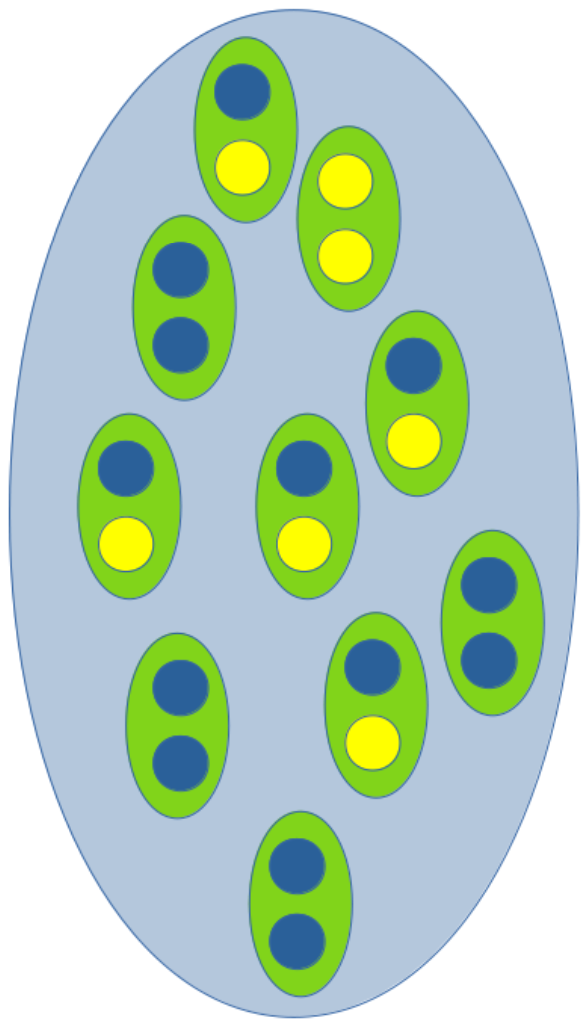
\includegraphics[width=.8\textwidth]{graphics_day2a_popgen/alleles_in_population.png}
		\end{center}
	\end{column}
	\begin{column}{.7\textwidth}
		\begin{itemize}
			\item Some individuals leave many offspring, others fewer, others none.
\visible<2->{\item Heterozygous individuals will randomly transmit allele $A$ or $a$.}
\visible<3->{\item It is likely that allele frequencies will change \emph{slightly} from one generation to another.}
\visible<4->{\item Over many generations, this process can produce large changes in allele frequencies.}
		\end{itemize}
	\end{column}
	\end{columns}
\end{frame}
%%%%%%%%%%%%%%%%%%%%%%%%%%%%%%%%%%%%%%%%%%%%%%%%%%%%%%%%%%%%%%%%%%%%%%%%%%%%%%%%%%%%%%
%
%
%
%%%%%%%%%%%%%%%%%%%%%%%%%%%%%%%%%%%%%%%%%%%%%%%%%%%%%%%%%%%%%%%%%%%%%%%%%%%%%%%%%%%%%%
\begin{frame}\frametitle{Model of genetic drift}
	We model the changes in allele frequency due to drift in a population using the \textbf{Wright-Fisher model}, which has the following assumptions:
	\begin{itemize}
		\item Haploid population.
		\item Asexual (no mating).
		\item Discrete generations.
	\end{itemize}
	\begin{block}{}
		The next generation of gene copies (or gametes) is produced by random \textbf{sampling with replacement} (independently and with equal probability) of gene copies from the previous generation.
	\end{block}
\end{frame}
%%%%%%%%%%%%%%%%%%%%%%%%%%%%%%%%%%%%%%%%%%%%%%%%%%%%%%%%%%%%%%%%%%%%%%%%%%%%%%%%%%%%%%
%
%
%
%%%%%%%%%%%%%%%%%%%%%%%%%%%%%%%%%%%%%%%%%%%%%%%%%%%%%%%%%%%%%%%%%%%%%%%%%%%%%%%%%%%%%%
\begin{frame}\frametitle{Model of genetic drift}
	\begin{figure}
	\begin{center}
		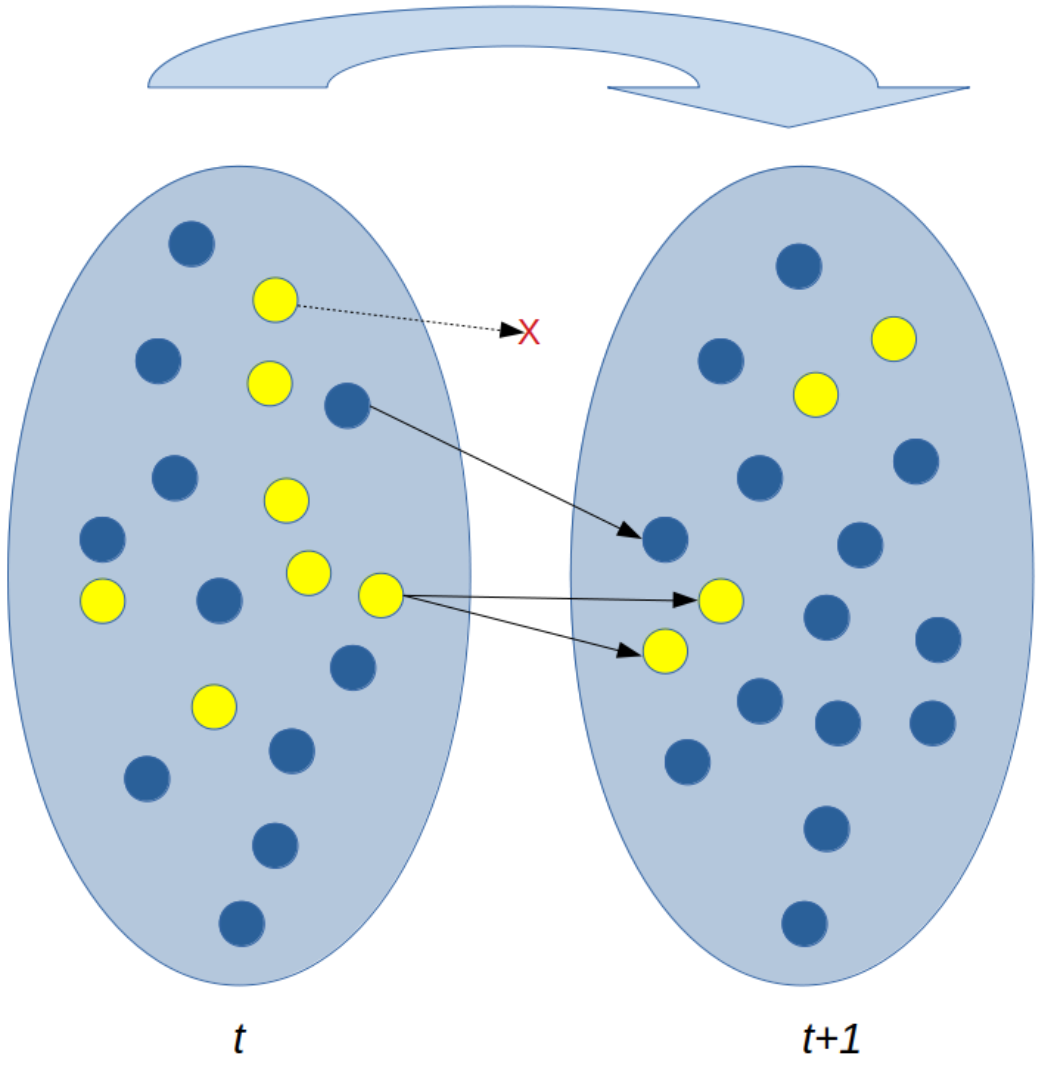
\includegraphics[width=.45\textwidth]{graphics_day2a_popgen/one_drift_step.png}
	\end{center}
	\caption{One generation of genetic drift.}
	\end{figure}
\only<1>{What is the \emph{expected} allele frequency in the next generation under this model? Do the experiment yourself!}
\only<2>{The \emph{expected} allele frequency in the next generation is equal to the allele frequency in the current generation.}
\end{frame}
%%%%%%%%%%%%%%%%%%%%%%%%%%%%%%%%%%%%%%%%%%%%%%%%%%%%%%%%%%%%%%%%%%%%%%%%%%%%%%%%%%%%%%
%
%
%
%%%%%%%%%%%%%%%%%%%%%%%%%%%%%%%%%%%%%%%%%%%%%%%%%%%%%%%%%%%%%%%%%%%%%%%%%%%%%%%%%%%%%
\begin{frame}\frametitle{Model of genetic drift}
	\begin{itemize}
		\item By pure chance we might sample a particular allele more or less often, causing the allele frequency to \emph{slightly} change from one generation to the next.
		\item Nevertheless, the \emph{expected} allele frequency in the next generation is equal to the allele frequency in the current generation.
	\end{itemize}
	\vspace{2ex}Why are these two apparently contradictory statements both true?
\end{frame}
%%%%%%%%%%%%%%%%%%%%%%%%%%%%%%%%%%%%%%%%%%%%%%%%%%%%%%%%%%%%%%%%%%%%%%%%%%%%%%%%%%%%%%
%
%
%
%%%%%%%%%%%%%%%%%%%%%%%%%%%%%%%%%%%%%%%%%%%%%%%%%%%%%%%%%%%%%%%%%%%%%%%%%%%%%%%%%%%%%
\begin{frame}\frametitle{Model of genetic drift}
	\begin{itemize}
		\item The distribution of offspring in generation $t + 1$ is given by a \textbf{binomial} distribution.
		\item Under the Wright-Fisher model, we can easily characterize the change in allele frequency mathematically.
	\end{itemize}
	\vspace{2ex}E.g. what is the probability that any gene copy in generation $t + 1$ is $A$?
\end{frame}
%%%%%%%%%%%%%%%%%%%%%%%%%%%%%%%%%%%%%%%%%%%%%%%%%%%%%%%%%%%%%%%%%%%%%%%%%%%%%%%%%%%%%%
%
%
%
%%%%%%%%%%%%%%%%%%%%%%%%%%%%%%%%%%%%%%%%%%%%%%%%%%%%%%%%%%%%%%%%%%%%%%%%%%%%%%%%%%%%%
\begin{frame}\frametitle{Expected allele frequency}
	What is the probability that any gene copy in generation $t + 1$ is $A$?
	\begin{equation}
		\E[f_A(t+1)] = 2N f_A(t)/2N = f_A(t)
	\end{equation}
	\begin{block}{}
		The expected allele frequency in generation $t + 1$ is equal to the allele frequency in generation $t$.
	\end{block}
\end{frame}
%%%%%%%%%%%%%%%%%%%%%%%%%%%%%%%%%%%%%%%%%%%%%%%%%%%%%%%%%%%%%%%%%%%%%%%%%%%%%%%%%%%%%%
%
%
%
%%%%%%%%%%%%%%%%%%%%%%%%%%%%%%%%%%%%%%%%%%%%%%%%%%%%%%%%%%%%%%%%%%%%%%%%%%%%%%%%%%%%%
\begin{frame}\frametitle{Wright-Fisher model}
	\begin{itemize}
		\item What happens if we repeat the sampling with replacement scheme over \textbf{many} generations?
		\item Do allele frequencies change over time?
		\item Do they get lost or fixed and with what probability?
		\item What is the effect of the initial allele frequency?
	\end{itemize}
\end{frame}
%%%%%%%%%%%%%%%%%%%%%%%%%%%%%%%%%%%%%%%%%%%%%%%%%%%%%%%%%%%%%%%%%%%%%%%%%%%%%%%%%%%%%%
%
%
%
%%%%%%%%%%%%%%%%%%%%%%%%%%%%%%%%%%%%%%%%%%%%%%%%%%%%%%%%%%%%%%%%%%%%%%%%%%%%%%%%%%%%%
\begin{frame}\frametitle{Wright-Fisher model}
	\begin{itemize}
		\item In each generation, the allele frequency might change a bit.
		\item Small changes add up and, after many generations, the allele frequency may have changed substantially.
	\end{itemize}
	\begin{block}{}
		Many small changes may result in large evolutionary changes over sufficiently long periods of time.
	\end{block}
\end{frame}
%%%%%%%%%%%%%%%%%%%%%%%%%%%%%%%%%%%%%%%%%%%%%%%%%%%%%%%%%%%%%%%%%%%%%%%%%%%%%%%%%%%%%%
%
%
%
%%%%%%%%%%%%%%%%%%%%%%%%%%%%%%%%%%%%%%%%%%%%%%%%%%%%%%%%%%%%%%%%%%%%%%%%%%%%%%%%%%%%%
\begin{frame}\frametitle{Wright-Fisher model}
	\begin{itemize}
		\item Allele frequency may increase or decrease with equal probabilities.
		\item In some cases, the allele has become fixed ($f = 1$) or is lost ($f = 0$).
	\end{itemize}
	\begin{block}{}
		When an allele first has become fixed or is lost, its frequency cannot change anymore$^{*}$.
	\end{block}
	{\scriptsize  $^{*}$If we ignore the effect of mutation. In fact, in the absence of recurrent mutation, it can be shown mathematically that a new allele must eventually become fixed or be lost.}
\end{frame}
%%%%%%%%%%%%%%%%%%%%%%%%%%%%%%%%%%%%%%%%%%%%%%%%%%%%%%%%%%%%%%%%%%%%%%%%%%%%%%%%%%%%%%
%
%
%
%%%%%%%%%%%%%%%%%%%%%%%%%%%%%%%%%%%%%%%%%%%%%%%%%%%%%%%%%%%%%%%%%%%%%%%%%%%%%%%%%%%%%
\begin{frame}\frametitle{Effect of population size}
	\begin{enumerate}
		\item How \textbf{fast} can genetic drift change allele frequencies?
		\item Does it depend on the population size?
		\item If so, would genetic drift be stronger in a small population or in a large population?
	\end{enumerate}
\end{frame}
%%%%%%%%%%%%%%%%%%%%%%%%%%%%%%%%%%%%%%%%%%%%%%%%%%%%%%%%%%%%%%%%%%%%%%%%%%%%%%%%%%%%%%
%
%
%
%%%%%%%%%%%%%%%%%%%%%%%%%%%%%%%%%%%%%%%%%%%%%%%%%%%%%%%%%%%%%%%%%%%%%%%%%%%%%%%%%%%%%
\begin{frame}\frametitle{Effect of population size}
	Large changes in allele frequency are unlikely to happen in large populations, but they happen more easily by chance in small populations.\\[2ex]
	\begin{block}{}
		Genetic drift works much faster in small populations than in large populations.
	\end{block}
	\vspace{2ex}The effect of population size on genetic drift has important implications for our understanding of natural populations. Why?
\end{frame}
%%%%%%%%%%%%%%%%%%%%%%%%%%%%%%%%%%%%%%%%%%%%%%%%%%%%%%%%%%%%%%%%%%%%%%%%%%%%%%%%%%%%%%
%
%
%
%%%%%%%%%%%%%%%%%%%%%%%%%%%%%%%%%%%%%%%%%%%%%%%%%%%%%%%%%%%%%%%%%%%%%%%%%%%%%%%%%%%%%
\begin{frame}
	Drift can be particularly strong under a population \textbf{bottleneck}.
	\begin{block}{Bottleneck}
		Short period of time when the population size is very small and many alleles become either fixed or lost in the population. As a consequence, much of the population genetic variation is lost.
	\end{block}
	\begin{center}
		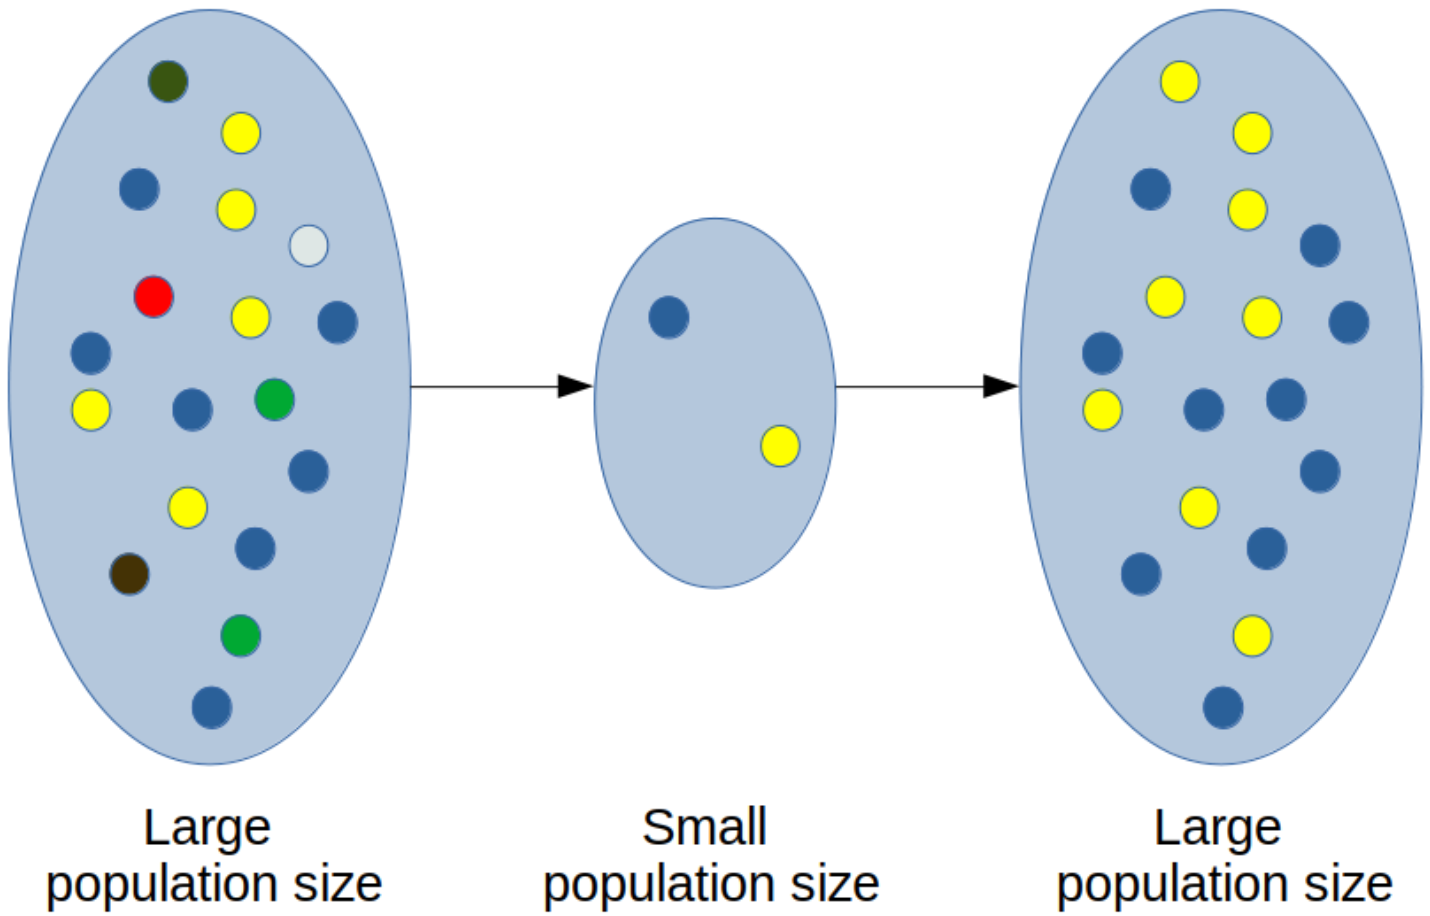
\includegraphics[width=.7\textwidth]{graphics_day2a_popgen/bottleneck.png}
	\end{center}
\end{frame}
%%%%%%%%%%%%%%%%%%%%%%%%%%%%%%%%%%%%%%%%%%%%%%%%%%%%%%%%%%%%%%%%%%%%%%%%%%%%%%%%%%%%%%
%
%
%
%%%%%%%%%%%%%%%%%%%%%%%%%%%%%%%%%%%%%%%%%%%%%%%%%%%%%%%%%%%%%%%%%%%%%%%%%%%%%%%%%%%%%
\begin{frame}\frametitle{Founder effect}
	\begin{block}{}
		Reduction in variability caused by a bottleneck in the population size during the founding of a new population.
	\end{block}
	\begin{center}
		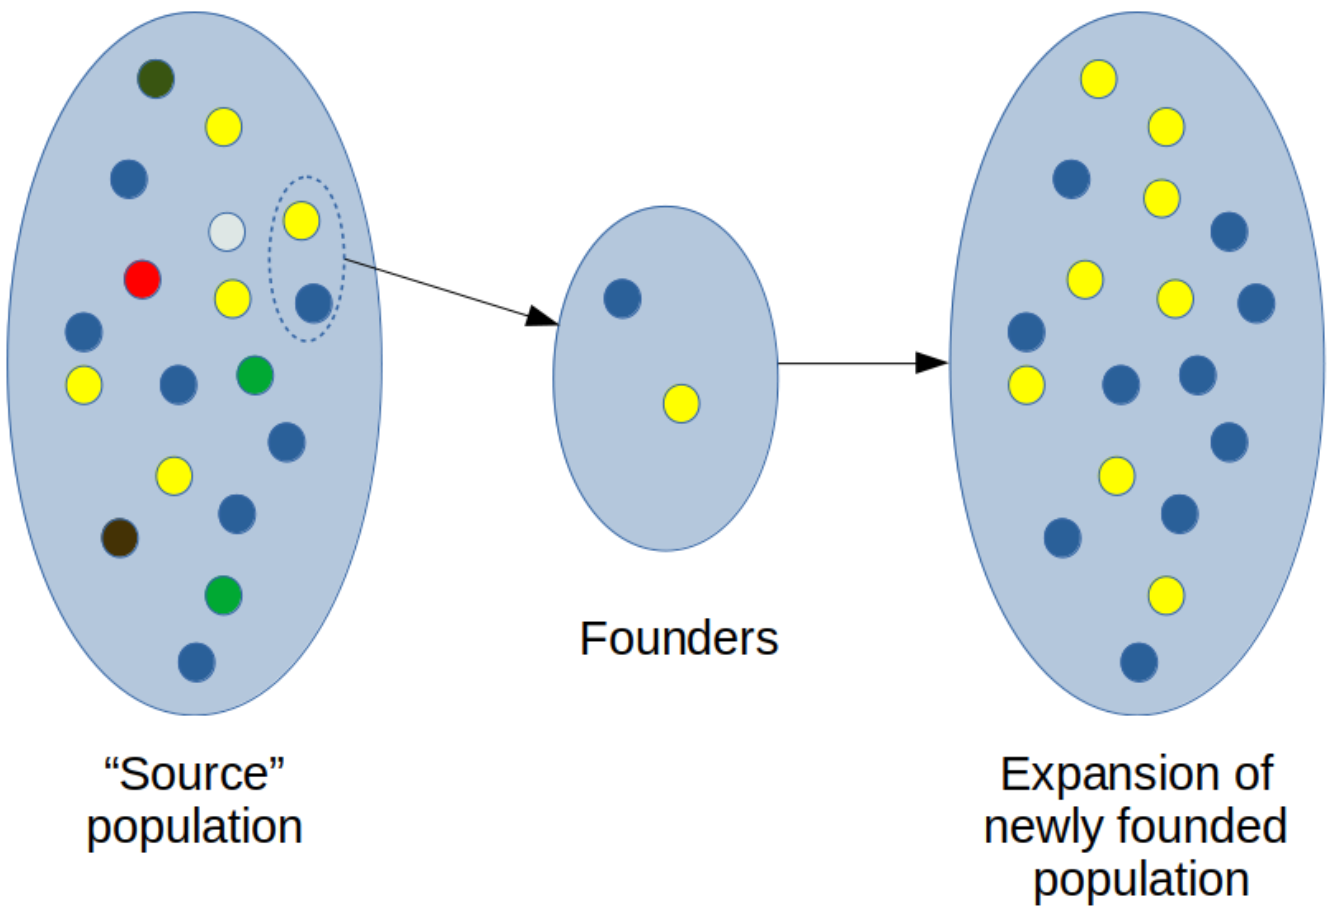
\includegraphics[width=.65\textwidth]{graphics_day2a_popgen/founder.png}
	\end{center}
\end{frame}
%%%%%%%%%%%%%%%%%%%%%%%%%%%%%%%%%%%%%%%%%%%%%%%%%%%%%%%%%%%%%%%%%%%%%%%%%%%%%%%%%%%%%%
%
%
%
%%%%%%%%%%%%%%%%%%%%%%%%%%%%%%%%%%%%%%%%%%%%%%%%%%%%%%%%%%%%%%%%%%%%%%%%%%%%%%%%%%%%%
\begin{frame}\frametitle{Founder effect}
	\begin{center}
		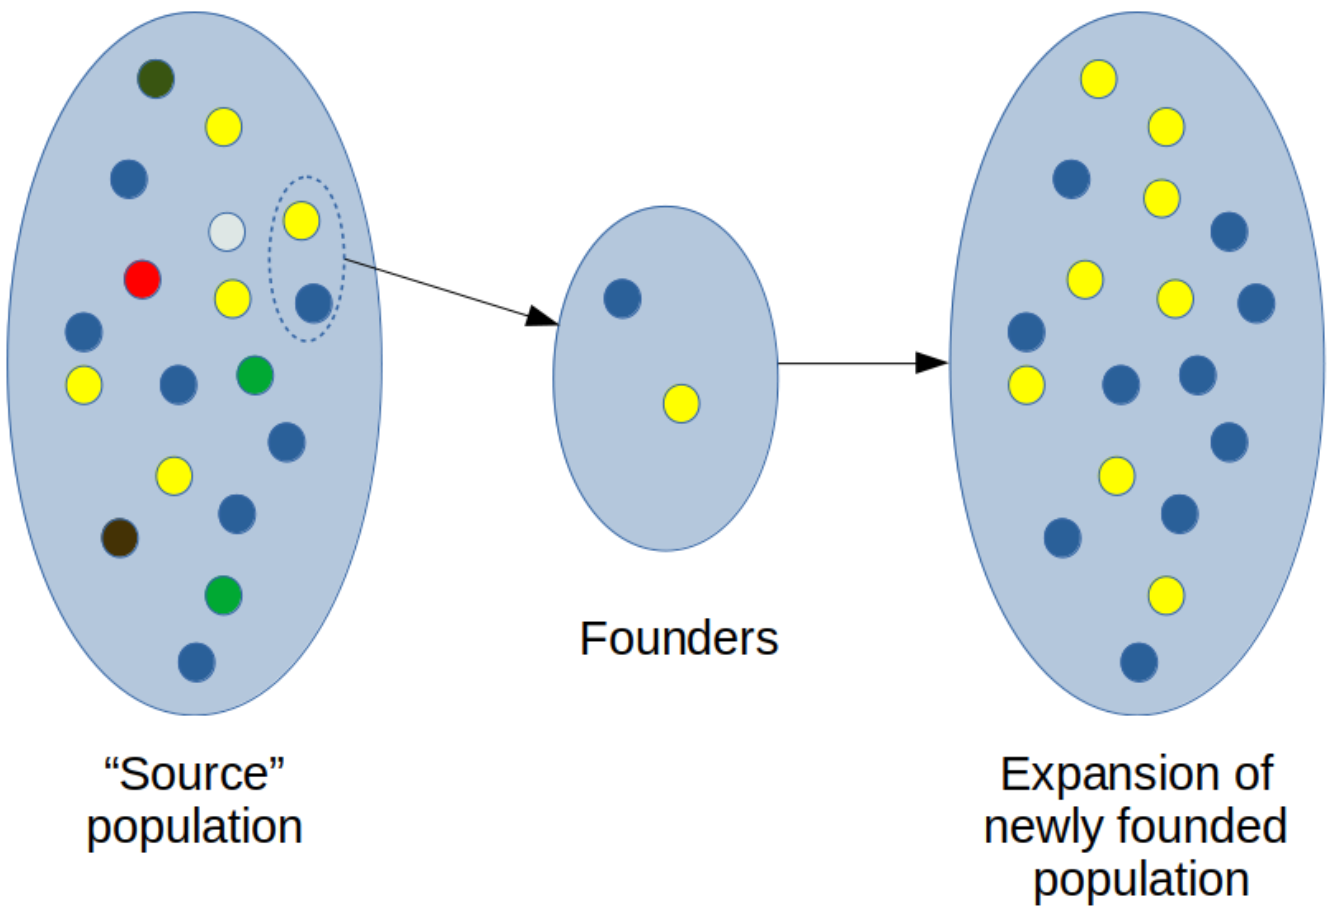
\includegraphics[width=.65\textwidth]{graphics_day2a_popgen/founder.png}
	\end{center}
	\begin{block}{}
		Genetic divergence after speciation may be helped along by the \textbf{strong} effects of genetic drift in the founders of a population.
	\end{block}
\end{frame}
%%%%%%%%%%%%%%%%%%%%%%%%%%%%%%%%%%%%%%%%%%%%%%%%%%%%%%%%%%%%%%%%%%%%%%%%%%%%%%%%%%%%%%
%
%
%
%%%%%%%%%%%%%%%%%%%%%%%%%%%%%%%%%%%%%%%%%%%%%%%%%%%%%%%%%%%%%%%%%%%%%%%%%%%%%%%%%%%%%
\begin{frame}\frametitle{Genetic drift}
	These models are an extremely simplified cartoon of ``real'' life. We could make it more realistic by allowing for:
	\begin{itemize}
		\item Two sexes.
		\item Population size to change over time.
		\item Number of offspring per individual to vary.
		\item ...
	\end{itemize}
	However, these modifications make little difference to the process of drift. The key fact is always true:
	\begin{block}{}
		Genetic drift causes allele frequencies to change in a random fashion over time.
	\end{block}
\end{frame}
%%%%%%%%%%%%%%%%%%%%%%%%%%%%%%%%%%%%%%%%%%%%%%%%%%%%%%%%%%%%%%%%%%%%%%%%%%%%%%%%%%%%%%
%
%
%
%%%%%%%%%%%%%%%%%%%%%%%%%%%%%%%%%%%%%%%%%%%%%%%%%%%%%%%%%%%%%%%%%%%%%%%%%%%%%%%%%%%%%
\begin{frame}\frametitle{So far so good}
	\begin{itemize}
		\item Random mating.
		\item Genetic drift.
	\end{itemize}
	\vspace{2.5ex}What if different alleles affect survival?
\end{frame}
%%%%%%%%%%%%%%%%%%%%%%%%%%%%%%%%%%%%%%%%%%%%%%%%%%%%%%%%%%%%%%%%%%%%%%%%%%%%%%%%%%%%%%
%
%
%
%%%%%%%%%%%%%%%%%%%%%%%%%%%%%%%%%%%%%%%%%%%%%%%%%%%%%%%%%%%%%%%%%%%%%%%%%%%%%%%%%%%%%
\begin{frame}\frametitle{Natural selection}
	\begin{itemize}
		\item Heritable traits that increase an individual's \textbf{fitness} become more common in the population.
		\item Mutations evolve accordingly to their \textbf{effect on the fitness} of the carrier.
		\item \textbf{Functionality} is the prerequisite for selection to be effective.
	\end{itemize}
	\phantom{pain}
	\begin{center}
		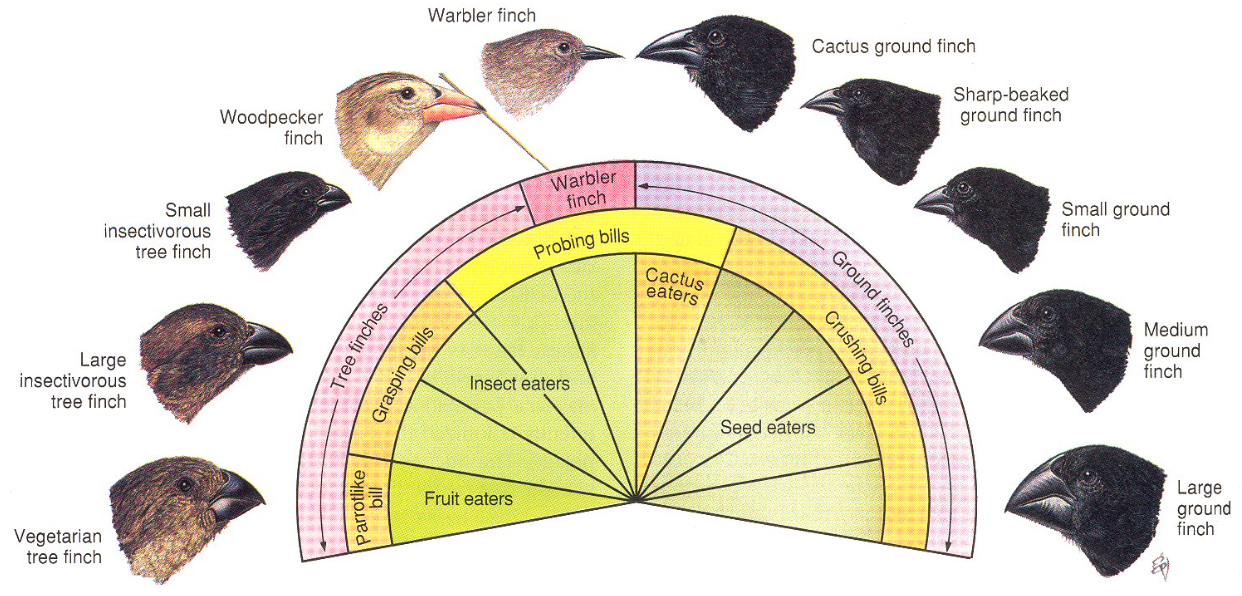
\includegraphics[width=.65\textwidth]{graphics_day2a_popgen/finches_with_beaks.png}
	\end{center}
\end{frame}
%%%%%%%%%%%%%%%%%%%%%%%%%%%%%%%%%%%%%%%%%%%%%%%%%%%%%%%%%%%%%%%%%%%%%%%%%%%%%%%%%%%%%%
%
%
%
%%%%%%%%%%%%%%%%%%%%%%%%%%%%%%%%%%%%%%%%%%%%%%%%%%%%%%%%%%%%%%%%%%%%%%%%%%%%%%%%%%%%%
\begin{frame}\frametitle{Fitness}
	We know that selection occurs because different individuals have different fitness, but what exactly do we mean by \textbf{fitness}?
\end{frame}
%%%%%%%%%%%%%%%%%%%%%%%%%%%%%%%%%%%%%%%%%%%%%%%%%%%%%%%%%%%%%%%%%%%%%%%%%%%%%%%%%%%%%%
%
%
%
%%%%%%%%%%%%%%%%%%%%%%%%%%%%%%%%%%%%%%%%%%%%%%%%%%%%%%%%%%%%%%%%%%%%%%%%%%%%%%%%%%%%%
\begin{frame}\frametitle{Fitness}
	The word fitness in an evolutionary context can be defined as:
	\begin{block}{}
		The expectation of the number of descendant genes at the same stage of the life cycle in the next generation.
	\end{block}
	\vspace{1ex}{\footnotesize In the next part, I will use \emph{fitness} to indicate a property of genotypes, not of alleles or phenotypes.}
\end{frame}
%%%%%%%%%%%%%%%%%%%%%%%%%%%%%%%%%%%%%%%%%%%%%%%%%%%%%%%%%%%%%%%%%%%%%%%%%%%%%%%%%%%%%%
%
%
%
%%%%%%%%%%%%%%%%%%%%%%%%%%%%%%%%%%%%%%%%%%%%%%%%%%%%%%%%%%%%%%%%%%%%%%%%%%%%%%%%%%%%%
\begin{frame}\frametitle{Absolute and relative fitness}
	\begin{itemize}
		\item \textbf{Absolute fitness}: measured as the change in abundance of a genotype from one generation to the next (assuming infinite population size, no mutation, and non-overlapping generations). In other words, the fittest genotypes will increase in abundance compared to less fit genotypes.
\visible<2>{\item \textbf{Relative fitness}: calculated by dividing all fitness values by the largest value, meaning the fittest genotype always has a relative fitness of 1.}
	\end{itemize}
\end{frame}
%%%%%%%%%%%%%%%%%%%%%%%%%%%%%%%%%%%%%%%%%%%%%%%%%%%%%%%%%%%%%%%%%%%%%%%%%%%%%%%%%%%%%%
%
%
%
%%%%%%%%%%%%%%%%%%%%%%%%%%%%%%%%%%%%%%%%%%%%%%%%%%%%%%%%%%%%%%%%%%%%%%%%%%%%%%%%%%%%%
\begin{frame}\frametitle{Fitness and selection}
	\begin{itemize}
		\item Fitness is a property of a particular genotype.
		\item Selection is a process leading to different expectations of how gene copies are transmitted to the next generation.
	\end{itemize}
	\vspace{2ex}If different individuals of a population have different fitness then we say that selection is operating.\\[2ex]
	If different individuals have the same fitness then we say that there is no selection, or equivalently, that the population is evolving \textbf{neutrally}.
\end{frame}
%%%%%%%%%%%%%%%%%%%%%%%%%%%%%%%%%%%%%%%%%%%%%%%%%%%%%%%%%%%%%%%%%%%%%%%%%%%%%%%%%%%%%%
%
%
%
%%%%%%%%%%%%%%%%%%%%%%%%%%%%%%%%%%%%%%%%%%%%%%%%%%%%%%%%%%%%%%%%%%%%%%%%%%%%%%%%%%%%%
\begin{frame}\frametitle{Fitness and selection}
	We need to consider the \textbf{fitness} of each genotype.\\[2ex]
	For example, for one locus with two alleles $A$ and $a$ in a diploid, each genotype has its fitness:
	\begin{itemize}
		\item $w_{AA}$ for genotype $AA$.
		\item $w_{Aa}$ for genotype $Aa$.
		\item $w_{aa}$ for genotype $aa$.
	\end{itemize}
\end{frame}
%%%%%%%%%%%%%%%%%%%%%%%%%%%%%%%%%%%%%%%%%%%%%%%%%%%%%%%%%%%%%%%%%%%%%%%%%%%%%%%%%%%%%%
%
%
%
%%%%%%%%%%%%%%%%%%%%%%%%%%%%%%%%%%%%%%%%%%%%%%%%%%%%%%%%%%%%%%%%%%%%%%%%%%%%%%%%%%%%%
\begin{frame}\frametitle{Fitness and selection}
	The strength of selection (or \textbf{selection coefficient}), often represented by the symbol $s$, is defined from the fitness values.\\[2ex]
	For example, if $Aa$ is not the fittest genotype then the selection coefficient against heterozygotes can be interpreted as the deficit from a relative fitness of 1, so that
	\begin{equation}
		w_{Aa} = 1-s
	\end{equation}
	What is the effect of selection on changes in allele frequency?
\end{frame}
%%%%%%%%%%%%%%%%%%%%%%%%%%%%%%%%%%%%%%%%%%%%%%%%%%%%%%%%%%%%%%%%%%%%%%%%%%%%%%%%%%%%%%
%
%
%
%%%%%%%%%%%%%%%%%%%%%%%%%%%%%%%%%%%%%%%%%%%%%%%%%%%%%%%%%%%%%%%%%%%%%%%%%%%%%%%%%%%%%
\begin{frame}\frametitle{Selection and drift combined}
	\begin{columns}
	\begin{column}{.5\textwidth}
		\begin{center}
			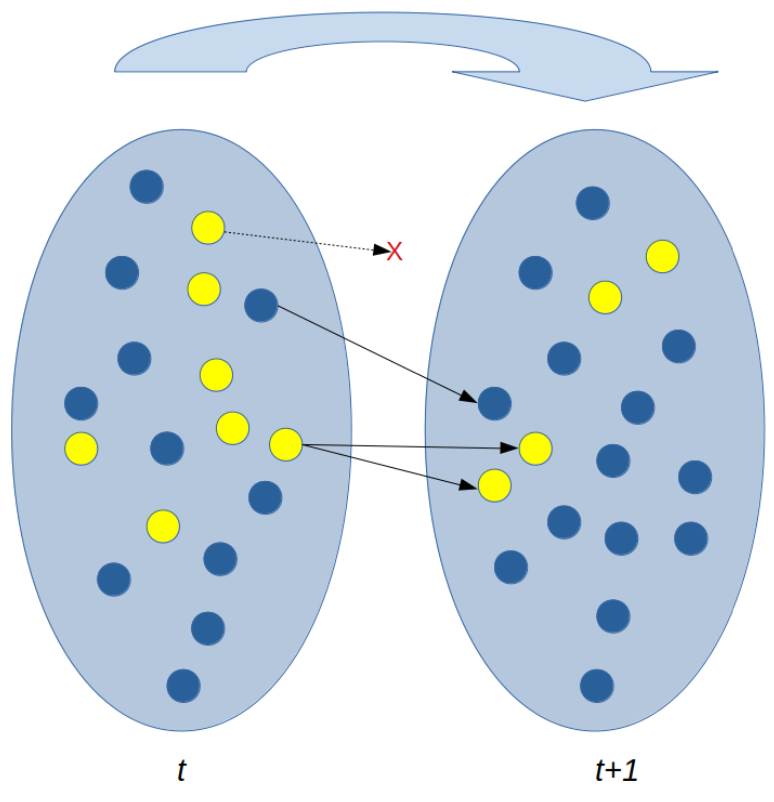
\includegraphics[width=.85\textwidth]{graphics_day2a_popgen/selection_and_drift.png}
		\end{center}		
	\end{column}
	\begin{column}{.5\textwidth}
		With drift only, all individuals had the same fitness.\\[1.5ex]
		The effect of high fitness is to make an individual more likely to be the parent of offspring in the next generation.\\[1.5ex]
		Nevertheless, it is still possible that a fit individual will have no offspring.
	\end{column}
	\end{columns}
\end{frame}
%%%%%%%%%%%%%%%%%%%%%%%%%%%%%%%%%%%%%%%%%%%%%%%%%%%%%%%%%%%%%%%%%%%%%%%%%%%%%%%%%%%%%%
%
%
%
%%%%%%%%%%%%%%%%%%%%%%%%%%%%%%%%%%%%%%%%%%%%%%%%%%%%%%%%%%%%%%%%%%%%%%%%%%%%%%%%%%%%%
\begin{frame}\frametitle{Selection and drift combined}
	If allele $A$ belongs to a genotype with high fitness, its frequency will still drift but with a ``tendency'' towards fixation.
	\begin{center}
		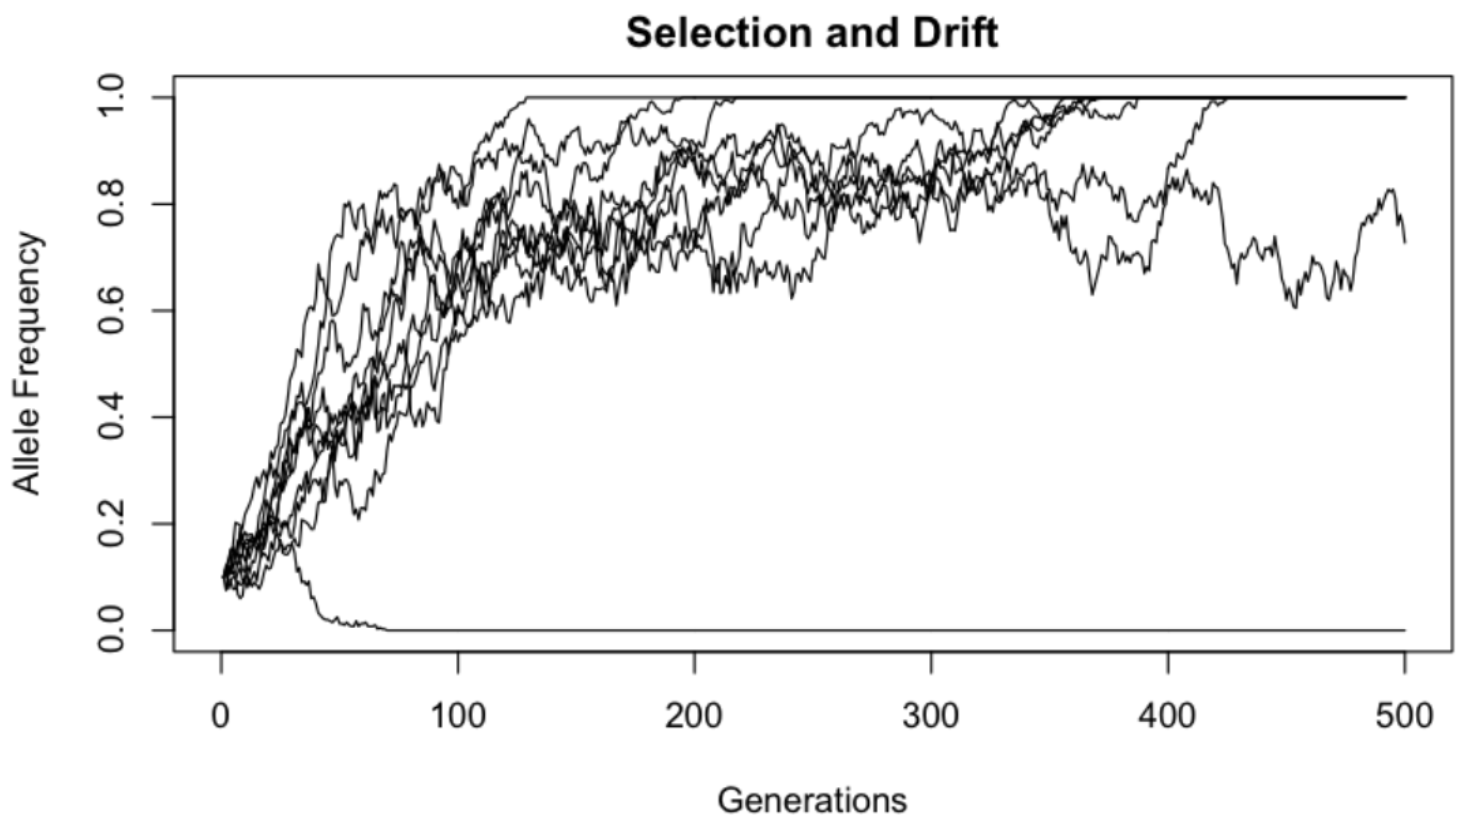
\includegraphics[width=.75\textwidth]{graphics_day2a_popgen/selection_and_drift_trajectory.png}
	\end{center}
	Is it still possible that the $A$ allele is lost?
\end{frame}
%%%%%%%%%%%%%%%%%%%%%%%%%%%%%%%%%%%%%%%%%%%%%%%%%%%%%%%%%%%%%%%%%%%%%%%%%%%%%%%%%%%%%%
%
%
%
%%%%%%%%%%%%%%%%%%%%%%%%%%%%%%%%%%%%%%%%%%%%%%%%%%%%%%%%%%%%%%%%%%%%%%%%%%%%%%%%%%%%%
\begin{frame}\frametitle{Intended Learning Outcomes}
	In this session you have learnt
	\begin{itemize}
		\item To describe genetic drift.
		\item To interpret the change of allele frequencies over time.
		\item To appreciate the effect of population size on drift.
		\item To define fitness and selection coefficient.
	\end{itemize}
\end{frame}
%%%%%%%%%%%%%%%%%%%%%%%%%%%%%%%%%%%%%%%%%%%%%%%%%%%%%%%%%%%%%%%%%%%%%%%%%%%%%%%%%%%%%%
%
%
%
%%%%%%%%%%%%%%%%%%%%%%%%%%%%%%%%%%%%%%%%%%%%%%%%%%%%%%%%%%%%%%%%%%%%%%%%%%%%%%%%%%%%%
\begin{frame}\frametitle{Intended Learning Outcomes}
	In this session you will learn
	\begin{itemize}
		\item To describe different types of natural selection.
		\item To appreciate the effect of novel mutations on allele frequency.
		\item To understand the concept of gene flow.
	\end{itemize}
\end{frame}
%%%%%%%%%%%%%%%%%%%%%%%%%%%%%%%%%%%%%%%%%%%%%%%%%%%%%%%%%%%%%%%%%%%%%%%%%%%%%%%%%%%%%%
%
%
%
%%%%%%%%%%%%%%%%%%%%%%%%%%%%%%%%%%%%%%%%%%%%%%%%%%%%%%%%%%%%%%%%%%%%%%%%%%%%%%%%%%%%%
\begin{frame}
	So far we have learnt how random mating and genetic drift change allele frequencies in time.\\
	What if
	\begin{itemize}
		\item Different alleles affect survival?
		\item New mutations arise?
		\item Migrants move between populations?
	\end{itemize}
\end{frame}
%%%%%%%%%%%%%%%%%%%%%%%%%%%%%%%%%%%%%%%%%%%%%%%%%%%%%%%%%%%%%%%%%%%%%%%%%%%%%%%%%%%%%%
%
%
%
%%%%%%%%%%%%%%%%%%%%%%%%%%%%%%%%%%%%%%%%%%%%%%%%%%%%%%%%%%%%%%%%%%%%%%%%%%%%%%%%%%%%%
\begin{frame}
	In other words, what is the effect of
	\begin{itemize}
		\item \textbf{Selection}
		\item Mutation
		\item Gene flow
	\end{itemize}
	on the change of allele frequency?
\end{frame}
%%%%%%%%%%%%%%%%%%%%%%%%%%%%%%%%%%%%%%%%%%%%%%%%%%%%%%%%%%%%%%%%%%%%%%%%%%%%%%%%%%%%%%
%
%
%
%%%%%%%%%%%%%%%%%%%%%%%%%%%%%%%%%%%%%%%%%%%%%%%%%%%%%%%%%%%%%%%%%%%%%%%%%%%%%%%%%%%%%
\begin{frame}\frametitle{Types of selection}
	If an allele is \textbf{dominant} then the heterozygote has the same \emph{phenotype} as the homozygote for the dominant allele.
	\begin{center}
		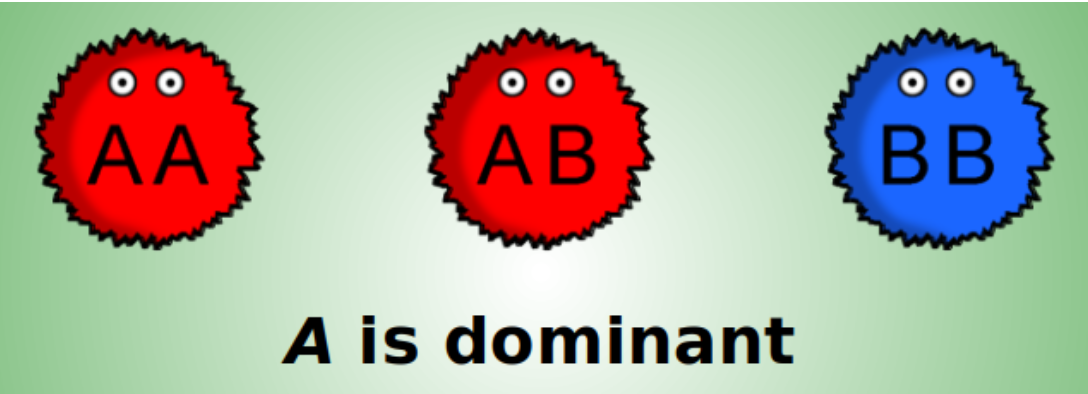
\includegraphics[width=.45\textwidth]{graphics_day2a_popgen/dominant_blobs.png}
	\end{center}
\visible<2>{If an allele is \textbf{recessive} then the heterozygote has the same \emph{phenotype} as the other homozygote.
	\begin{center}
		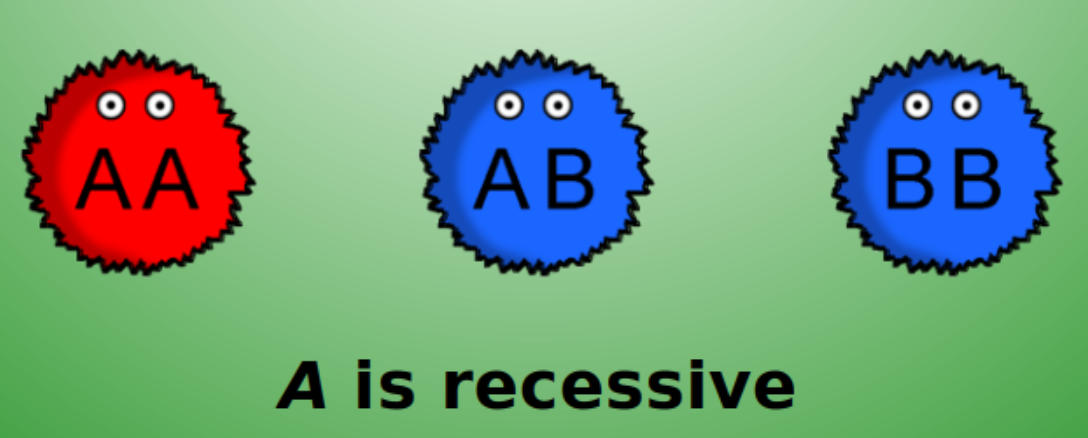
\includegraphics[width=.45\textwidth]{graphics_day2a_popgen/recessive_blobs.png}
	\end{center}}
\end{frame}
%%%%%%%%%%%%%%%%%%%%%%%%%%%%%%%%%%%%%%%%%%%%%%%%%%%%%%%%%%%%%%%%%%%%%%%%%%%%%%%%%%%%%%
%
%
%
%%%%%%%%%%%%%%%%%%%%%%%%%%%%%%%%%%%%%%%%%%%%%%%%%%%%%%%%%%%%%%%%%%%%%%%%%%%%%%%%%%%%%
\begin{frame}\frametitle{Types of selection}
	If $A$ is \textbf{dominant} then the heterozygote has the same \emph{fitness} as the homozygote for that allele.
	\begin{center}
		
\includegraphics[width=.45\textwidth]{graphics_day2a_popgen/dominant_blobs_arms.png}
	\end{center}
\visible<2>{If an allele is \textbf{recessive} then the heterozygote has the same \emph{fitness} as the other homozygote.
	\begin{center}
		
\includegraphics[width=.45\textwidth]{graphics_day2a_popgen/recessive_blobs_arms.png}
	\end{center}}
\end{frame}
%%%%%%%%%%%%%%%%%%%%%%%%%%%%%%%%%%%%%%%%%%%%%%%%%%%%%%%%%%%%%%%%%%%%%%%%%%%%%%%%%%%%%%
%
%
%
%%%%%%%%%%%%%%%%%%%%%%%%%%%%%%%%%%%%%%%%%%%%%%%%%%%%%%%%%%%%%%%%%%%%%%%%%%%%%%%%%%%%%
\begin{frame}
	\begin{block}{}
		The \textbf{selection coefficient} $s$ is defined as $\tfrac{w_a}{w_A} = 1 - s$ for haploids with alleles $A$ and $a$, with $A$ being fitter.
	\end{block}
\visible<2>{$f_A(t)$ depends approximately on the product between $s$ (selection coefficient, or ``strength'') and t (time):\\[1ex]
	If $s$ is small, then the value of $t$ to generate a certain change in $f_A$ is \emph{inversely} proportional to s.\\[2ex]
	If $s > 0$ then $A$-bearing individuals have the advantage, the opposite is true for $s < 0$.}
\end{frame}
%%%%%%%%%%%%%%%%%%%%%%%%%%%%%%%%%%%%%%%%%%%%%%%%%%%%%%%%%%%%%%%%%%%%%%%%%%%%%%%%%%%%%%
%
%
%
%%%%%%%%%%%%%%%%%%%%%%%%%%%%%%%%%%%%%%%%%%%%%%%%%%%%%%%%%%%%%%%%%%%%%%%%%%%%%%%%%%%%%
\begin{frame}\frametitle{Additive selection}
	What if a recessive allele is not totally masked by the dominant allele?
	\begin{center}
		
\includegraphics[width=.45\textwidth]{graphics_day2a_popgen/dominant_blobs_arms.png}
	\end{center}
	If the trait affected by $A$ has additive fitness then the heterozygote has a fitness value that is intermediate between the two homozygotes$^{*}$.\\[2ex]
	{\scriptsize $^{*}$You do not need to know any more than that. This enters an area called \emph{quantitative genetics} and there are entire courses on that topic.}
\end{frame}
%%%%%%%%%%%%%%%%%%%%%%%%%%%%%%%%%%%%%%%%%%%%%%%%%%%%%%%%%%%%%%%%%%%%%%%%%%%%%%%%%%%%%%
%
%
%
%%%%%%%%%%%%%%%%%%%%%%%%%%%%%%%%%%%%%%%%%%%%%%%%%%%%%%%%%%%%%%%%%%%%%%%%%%%%%%%%%%%%%
\begin{frame}\frametitle{Types of selection}
	The types of selection just described can be defined as:
	\begin{itemize}
		\item Additive selection: $w_{AA} = 1$; $w_{Aa} = 1-s$; $w_{aa} = 1-2s$.
		\item Dominant advantageous allele: $w_{AA} = w_{Aa} > w_{aa}$.
		\item Recessive advantageous allele: $w_{AA} > w_{Aa} = w_{aa}$.
	\end{itemize}
	with $A$ being the advantageous allele.
\end{frame}
%%%%%%%%%%%%%%%%%%%%%%%%%%%%%%%%%%%%%%%%%%%%%%%%%%%%%%%%%%%%%%%%%%%%%%%%%%%%%%%%%%%%%%
%
%
%
%%%%%%%%%%%%%%%%%%%%%%%%%%%%%%%%%%%%%%%%%%%%%%%%%%%%%%%%%%%%%%%%%%%%%%%%%%%%%%%%%%%%%
\begin{frame}
	If the selection coefficient does not change over time, we have several possible scenarios:
	\begin{itemize}
		\item \textbf{Directional} selection (additive, dominant or recessive): One allele is favoured.
		\item \textbf{Heterozygote advantage}: Special case of balancing selection where multiple alleles are maintained in the population.
		\item \textbf{Heterozygote disadvantage}: Special case of disruptive selection where the extremes of a trait are favoured.
		\item \textbf{Stabilising selection}: Variation is reduced.
	\end{itemize}
	\begin{center}
		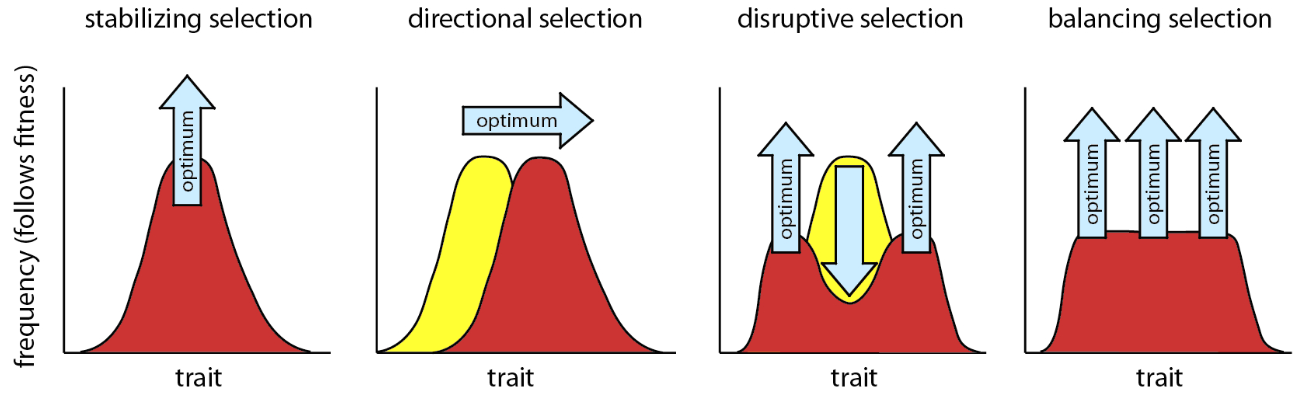
\includegraphics[width=.45\textwidth]{graphics_day2a_popgen/polygenic_selection_models.png}
	\end{center}
	{\footnotesize If the direction of selection changes over time, we have fluctuating selection.}
\end{frame}
%%%%%%%%%%%%%%%%%%%%%%%%%%%%%%%%%%%%%%%%%%%%%%%%%%%%%%%%%%%%%%%%%%%%%%%%%%%%%%%%%%%%%%
%
%
%
%%%%%%%%%%%%%%%%%%%%%%%%%%%%%%%%%%%%%%%%%%%%%%%%%%%%%%%%%%%%%%%%%%%%%%%%%%%%%%%%%%%%%%
\begin{frame}\frametitle{Directional selection}
	$A$ is the advantageous allele if $w_{aa} \leq w_{Aa} \leq w_{AA}$.\\[2ex]
	$f_A$ will increase every generation and eventually reach 1 (i.e.\ \textbf{fixation} of $A$ and \textbf{loss} of $a$).\\[2ex]
	The rate of change in allele frequency depends on $s$, the selection coefficient.\\
	Even small $s$ can change allele frequency substantially over many generations.
\end{frame}
%%%%%%%%%%%%%%%%%%%%%%%%%%%%%%%%%%%%%%%%%%%%%%%%%%%%%%%%%%%%%%%%%%%%%%%%%%%%%%%%%%%%%%
%
%
%
%%%%%%%%%%%%%%%%%%%%%%%%%%%%%%%%%%%%%%%%%%%%%%%%%%%%%%%%%%%%%%%%%%%%%%%%%%%%%%%%%%%%%%
\begin{frame}\frametitle{Heterozygote advantage}
	If $w_{Aa} > w_{AA}, w_{aa}$ we define
	\begin{equation}
		\begin{split}
			\tfrac{w_{aa}}{w_{Aa}} & = 1 - s_{aa}\\
			\tfrac{w_{AA}}{w_{Aa}} & = 1 - s_{AA}
		\end{split}
	\end{equation}
	$f_A$ will tend to the same intermediate value regardless of its initial frequency. In fact, selection will not eliminate either allele (it is a special case of \textbf{balancing selection}).
\end{frame}
%%%%%%%%%%%%%%%%%%%%%%%%%%%%%%%%%%%%%%%%%%%%%%%%%%%%%%%%%%%%%%%%%%%%%%%%%%%%%%%%%%%%%%
%
%
%
%%%%%%%%%%%%%%%%%%%%%%%%%%%%%%%%%%%%%%%%%%%%%%%%%%%%%%%%%%%%%%%%%%%%%%%%%%%%%%%%%%%%%%
\begin{frame}\frametitle{Heterozygote disadvantage}
	If $w_{Aa} < w_{AA}, w_{aa}$, it results in the fixation of one of the two alleles (which one?).\\[2ex]
	It is an example of \textbf{disruptive selection} that removes low-minor-frequency alleles.
\end{frame}
%%%%%%%%%%%%%%%%%%%%%%%%%%%%%%%%%%%%%%%%%%%%%%%%%%%%%%%%%%%%%%%%%%%%%%%%%%%%%%%%%%%%%%
%
%
%
%%%%%%%%%%%%%%%%%%%%%%%%%%%%%%%%%%%%%%%%%%%%%%%%%%%%%%%%%%%%%%%%%%%%%%%%%%%%%%%%%%%%%%
\begin{frame}
	We have learnt how \textbf{selection} changes allele frequencies in time. You also know how \textbf{genetic drift} changes allele frequencies in time.
	\begin{block}{}
		What is the combined effect of selection and drift?
	\end{block}
\end{frame}
%%%%%%%%%%%%%%%%%%%%%%%%%%%%%%%%%%%%%%%%%%%%%%%%%%%%%%%%%%%%%%%%%%%%%%%%%%%%%%%%%%%%%%
%
%
%
%%%%%%%%%%%%%%%%%%%%%%%%%%%%%%%%%%%%%%%%%%%%%%%%%%%%%%%%%%%%%%%%%%%%%%%%%%%%%%%%%%%%%%
\begin{frame}
	For a population of size $N$, the fixation probability $u$ of a new mutation with selection coefficient $s$ can be defined as:
	\begin{itemize}
		\item Strongly deleterious: If $2Ns << -1$ then $u \approx 0$.
		\item Nearly neutral deleterious: If $-1 < 2Ns < 1$ then $u \approx 1/(2N)$.
		\item Strongly advantageous: If $2Ns >> 1$ then $u \approx 2s$.
	\end{itemize}
\end{frame}
%%%%%%%%%%%%%%%%%%%%%%%%%%%%%%%%%%%%%%%%%%%%%%%%%%%%%%%%%%%%%%%%%%%%%%%%%%%%%%%%%%%%%%
%
%
%
%%%%%%%%%%%%%%%%%%%%%%%%%%%%%%%%%%%%%%%%%%%%%%%%%%%%%%%%%%%%%%%%%%%%%%%%%%%%%%%%%%%%%%
\begin{frame}
	\begin{block}{}
		Strongly advantageous mutations are not necessarily fixed. Slightly deleterious alleles have a small but non-zero chance of being fixed.
	\end{block}
	\vspace{2ex}
	\begin{block}{}
		Whether an allele is strongly selected or nearly neutral depends on both the selection coefficient and the population size.
	\end{block}
\end{frame}
%%%%%%%%%%%%%%%%%%%%%%%%%%%%%%%%%%%%%%%%%%%%%%%%%%%%%%%%%%%%%%%%%%%%%%%%%%%%%%%%%%%%%%
%
%
%
%%%%%%%%%%%%%%%%%%%%%%%%%%%%%%%%%%%%%%%%%%%%%%%%%%%%%%%%%%%%%%%%%%%%%%%%%%%%%%%%%%%%%
\begin{frame}
	In other words, what is the effect of
	\begin{itemize}
		\item Selection
		\item \textbf{Mutation}
		\item Gene flow
	\end{itemize}
	on the change of allele frequency?
\end{frame}
%%%%%%%%%%%%%%%%%%%%%%%%%%%%%%%%%%%%%%%%%%%%%%%%%%%%%%%%%%%%%%%%%%%%%%%%%%%%%%%%%%%%%%
%
%
%
%%%%%%%%%%%%%%%%%%%%%%%%%%%%%%%%%%%%%%%%%%%%%%%%%%%%%%%%%%%%%%%%%%%%%%%%%%%%%%%%%%%%%
\begin{frame}\frametitle{Mutations}
	New mutations arise to produce new genetic variation that genetic drift can act on:
	\begin{itemize}
		\item Deletions
		\item Insertions
		\item Translocations
		\item Point mutations
	\end{itemize}
	Any of these mutations can be represented with a bi-allelic model (e.g. presence/absence) if we assume that multiple mutations cannot occur in the same location$^{*}$.\\[2ex]
	{\footnotesize $^{*}$This assumption is also called the \emph{infinite} site model.}
\end{frame}
%%%%%%%%%%%%%%%%%%%%%%%%%%%%%%%%%%%%%%%%%%%%%%%%%%%%%%%%%%%%%%%%%%%%%%%%%%%%%%%%%%%%%%
%
%
%
%%%%%%%%%%%%%%%%%%%%%%%%%%%%%%%%%%%%%%%%%%%%%%%%%%%%%%%%%%%%%%%%%%%%%%%%%%%%%%%%%%%%%
\begin{frame}
	Assume that the yellow $a$ allele in each individual randomly mutates to blue $A$ with probability $\mu$ (called the \textbf{mutation rate}) in each generation.
	\begin{center}
		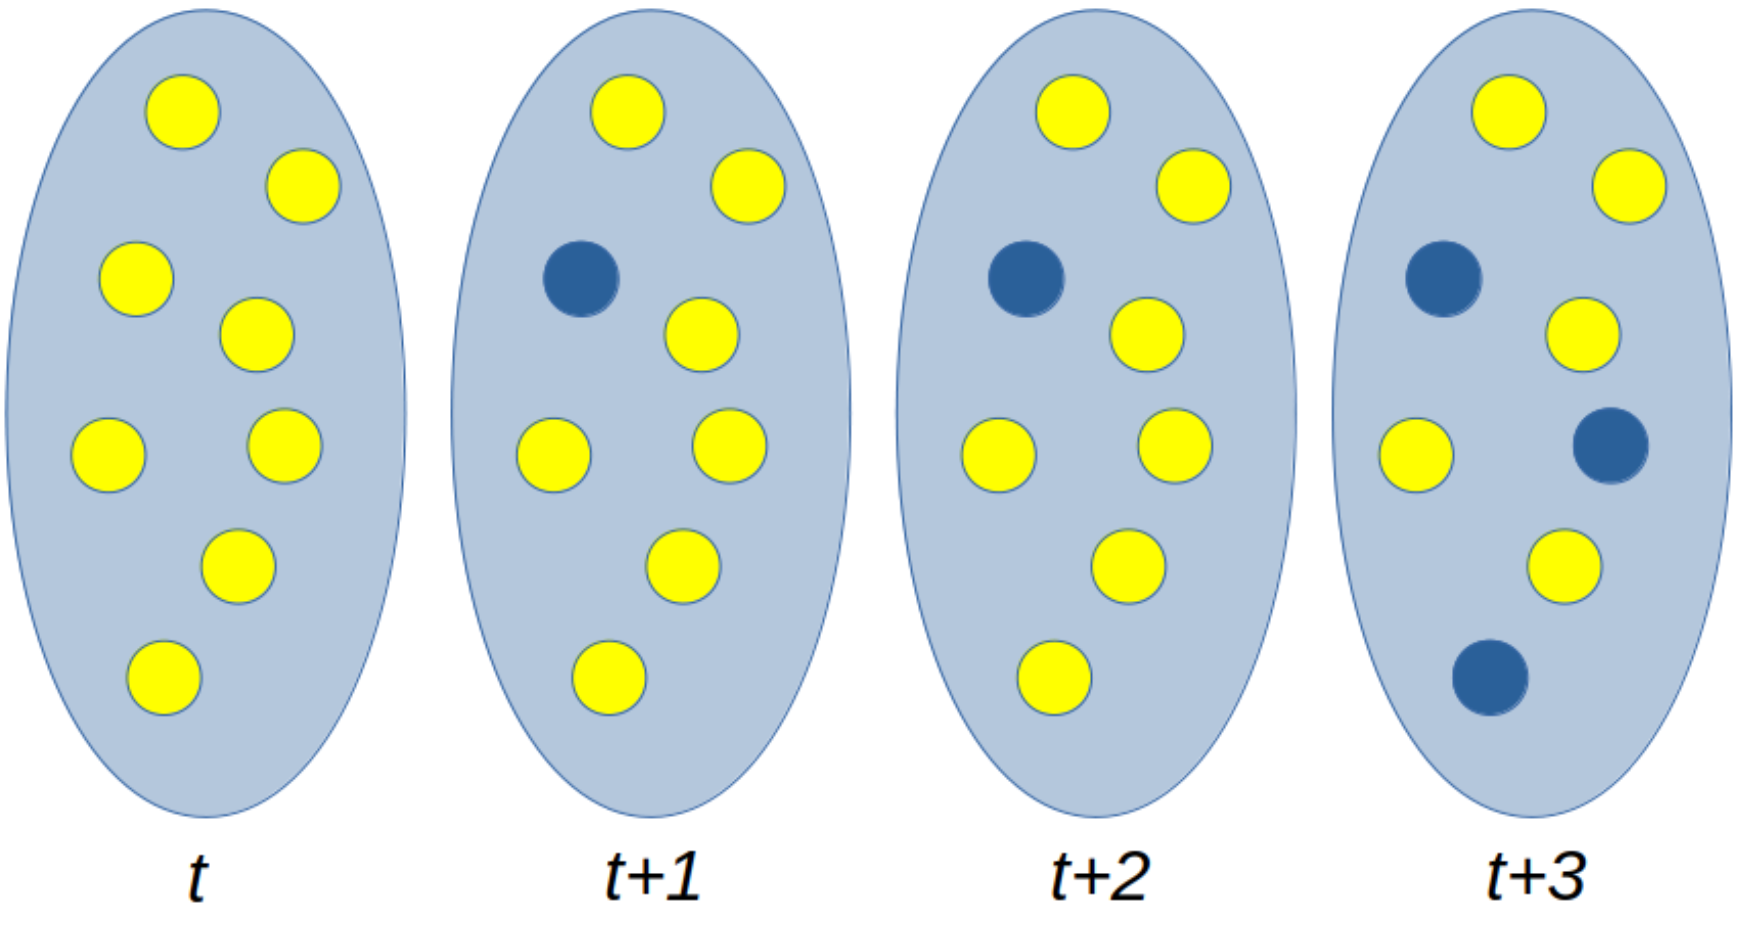
\includegraphics[width=.65\textwidth]{graphics_day2a_popgen/mutation_generations.png}
	\end{center}
\end{frame}
%%%%%%%%%%%%%%%%%%%%%%%%%%%%%%%%%%%%%%%%%%%%%%%%%%%%%%%%%%%%%%%%%%%%%%%%%%%%%%%%%%%%%%
%
%
%
%%%%%%%%%%%%%%%%%%%%%%%%%%%%%%%%%%%%%%%%%%%%%%%%%%%%%%%%%%%%%%%%%%%%%%%%%%%%%%%%%%%%%
\begin{frame}
	\begin{center}
		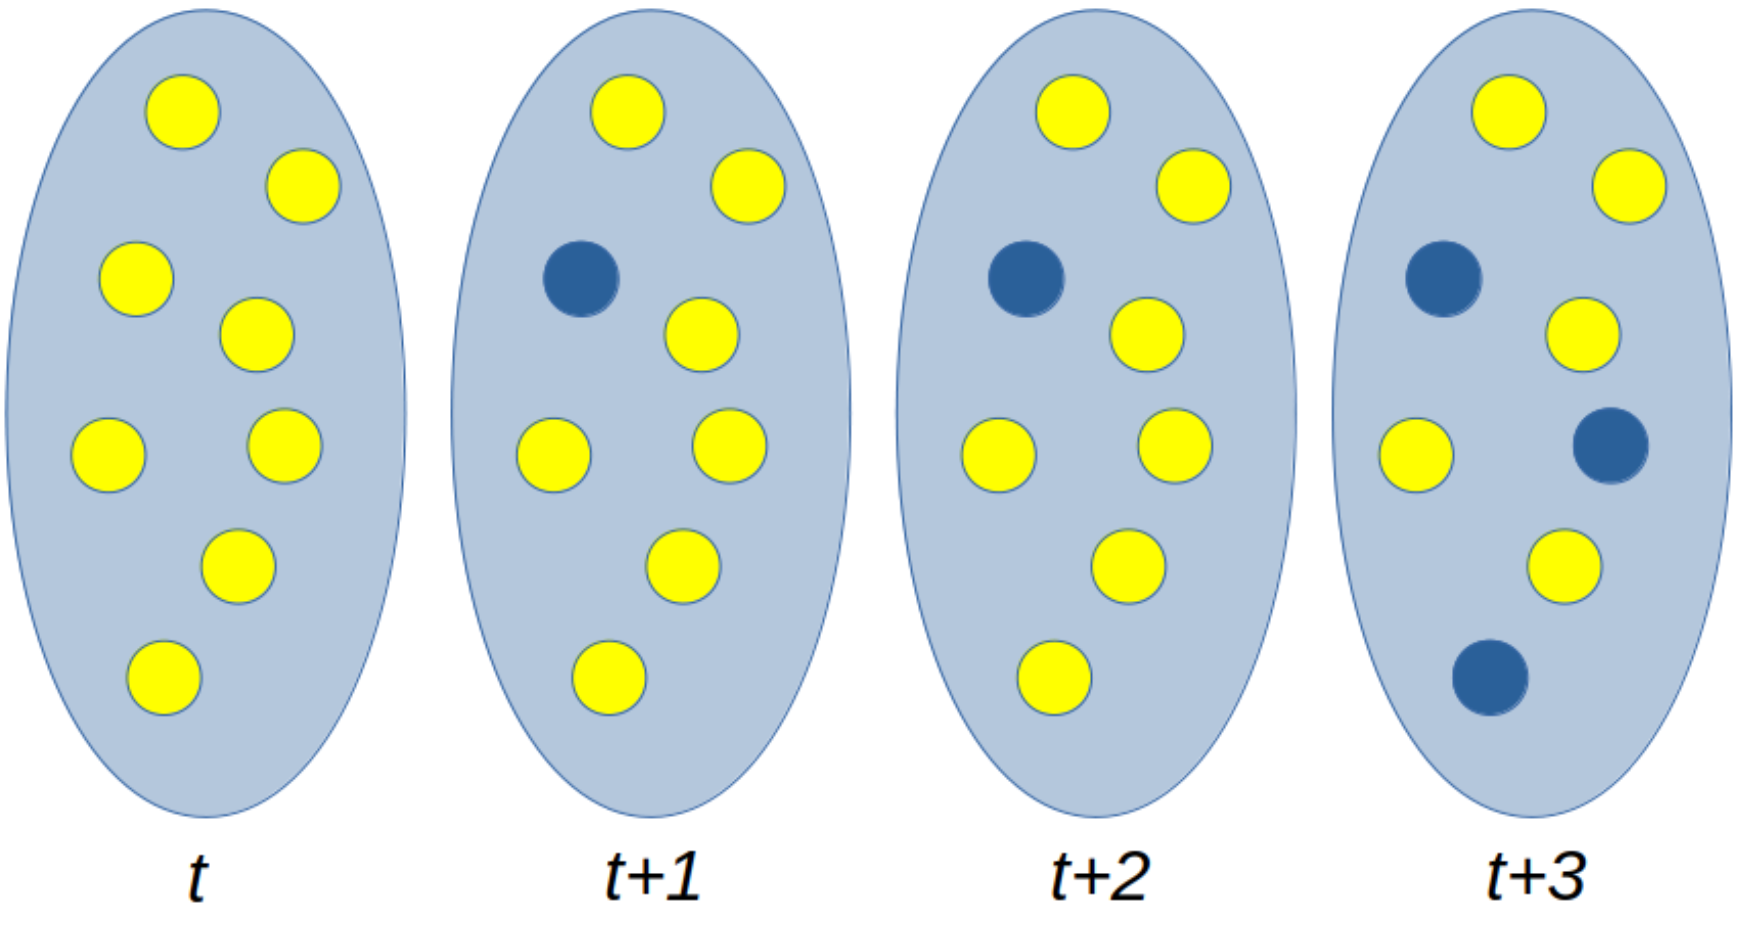
\includegraphics[width=.5\textwidth]{graphics_day2a_popgen/mutation_generations.png}
	\end{center}
% \only<1-2>{What is the expected allele frequency in the next generation given the current allele frequency of the mutation rate?
% \visible<2>{\vspace{2ex}In the absence of other forces (e.g.\ genetic drift and selection), an equilibrium will be reached at:
% 	\begin{equation}
% 		\frac{\text{mutation rate to blue}}{(\text{mutation rate to blue} + \text{mutation rate to yellow})}		
% 	\end{equation}}}
\only<1-3>{What is the expected allele frequency in the next generation $\E[f_A(t + 1)]$ given the current allele frequency $f_A(t)$ and the mutation rate $\mu$?
\visible<2-3>{\begin{equation}
		\E[f_A(t + 1)] = f_A(t) + \mu f_a(t)
	\end{equation}
	Why?\\}
\visible<3>{$f_A$ will increase by the number of alleles $a$ that mutate to $A$, given by the rate $\mu$ times the frequency of $a$ alleles to be mutated to $A$.}}
\only<4-5>{If mutations occur in both directions, e.g.\ mutations occur at rate $\mu_{a\to A}$ from $a$ to $A$ and $\mu_{A\to a}$ from $A$ to $a$, then
	\begin{equation}
		\E[f_A(t + 1)] = (1 - \mu_{A\to a})f_A(t) + \mu_{a\to A} f_a(t)
	\end{equation}
	Why?\\
\visible<5>{$f_A$ will increase by the number of alleles $a$ that mutate to $A$, but decrease by the number of alleles $A$ that mutate to $a$.}}
\only<6>{In the absence of other forces (e.g.\ genetic drift and selection), we can show that an equilibrium will eventually be established at:
	\begin{equation}
		f_A = \frac{\mu_{a\to A}}{\mu_{a\to A} + \mu_{A\to a}}
	\end{equation}}
\end{frame}
%%%%%%%%%%%%%%%%%%%%%%%%%%%%%%%%%%%%%%%%%%%%%%%%%%%%%%%%%%%%%%%%%%%%%%%%%%%%%%%%%%%%%%
%
%
%
%%%%%%%%%%%%%%%%%%%%%%%%%%%%%%%%%%%%%%%%%%%%%%%%%%%%%%%%%%%%%%%%%%%%%%%%%%%%%%%%%%%%%
\begin{frame}\frametitle{Mutation rate}
	\begin{center}
		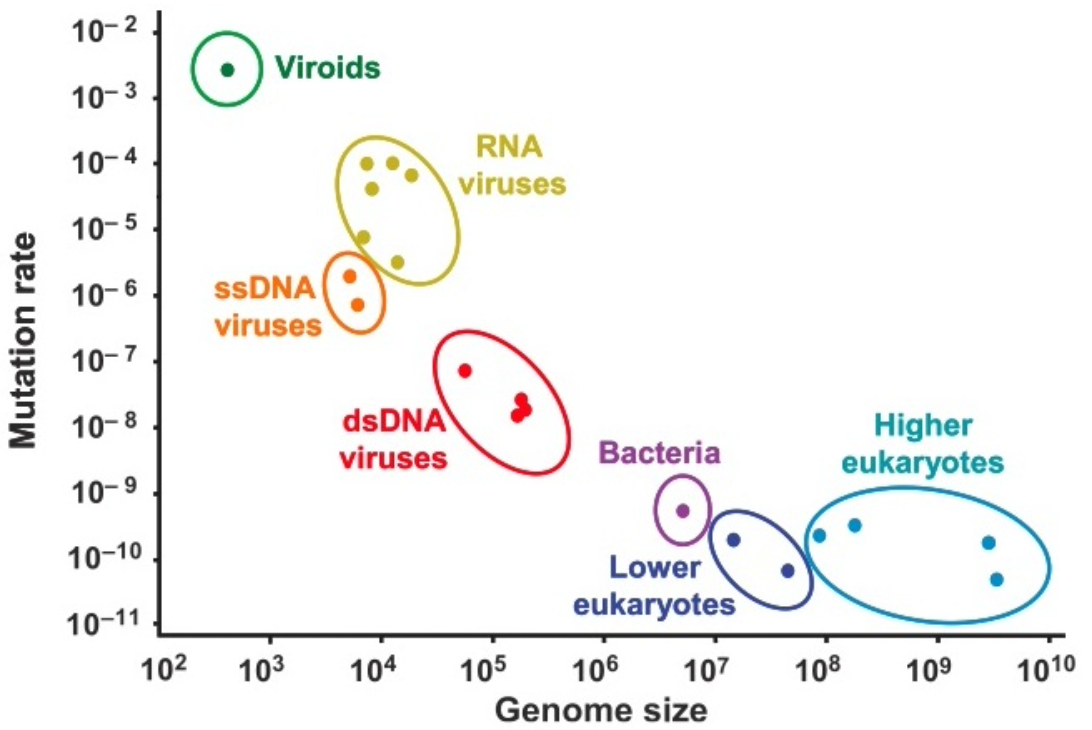
\includegraphics[width=.45\textwidth]{graphics_day2a_popgen/mutation_rate.png}
	\end{center}
	It is important to note that:
	\begin{itemize}
		\item Mutation is a weak force in higher organisms.
		\item With no genetic drift (and selection), it takes a long time for the allele frequency to reach equilibrium.
		\item We can often ignore recurrent mutations.
	\end{itemize}
\end{frame}
%%%%%%%%%%%%%%%%%%%%%%%%%%%%%%%%%%%%%%%%%%%%%%%%%%%%%%%%%%%%%%%%%%%%%%%%%%%%%%%%%%%%%%
%
%
%
%%%%%%%%%%%%%%%%%%%%%%%%%%%%%%%%%%%%%%%%%%%%%%%%%%%%%%%%%%%%%%%%%%%%%%%%%%%%%%%%%%%%%
\begin{frame}
	In other words, what is the effect of
	\begin{itemize}
		\item Selection
		\item Mutation
		\item \textbf{Gene flow}
	\end{itemize}
	on the change of allele frequency?
\end{frame}
%%%%%%%%%%%%%%%%%%%%%%%%%%%%%%%%%%%%%%%%%%%%%%%%%%%%%%%%%%%%%%%%%%%%%%%%%%%%%%%%%%%%%%
%
%
%
%%%%%%%%%%%%%%%%%%%%%%%%%%%%%%%%%%%%%%%%%%%%%%%%%%%%%%%%%%%%%%%%%%%%%%%%%%%%%%%%%%%%%
\begin{frame}\frametitle{Population subdivision}
	\begin{block}{}
		There is population subdivision, or \textbf{structure}, when the population is not randomly mating because of geographic or social structure.
	\end{block}
	\vspace{1.5ex}
	Population subdivision is important to
	\begin{itemize}
		\item Understand the effects of drift and natural selection.
		\item Plan conservation strategies for rare or endangered species.
	\end{itemize}
\end{frame}
%%%%%%%%%%%%%%%%%%%%%%%%%%%%%%%%%%%%%%%%%%%%%%%%%%%%%%%%%%%%%%%%%%%%%%%%%%%%%%%%%%%%%%
%
%
%
%%%%%%%%%%%%%%%%%%%%%%%%%%%%%%%%%%%%%%%%%%%%%%%%%%%%%%%%%%%%%%%%%%%%%%%%%%%%%%%%%%%%%
\begin{frame}\frametitle{Population subdivision}
	Let us assume that we have a population comprising of a certain number of individuals (i.e.\ diploid genotypes).
	\begin{center}
		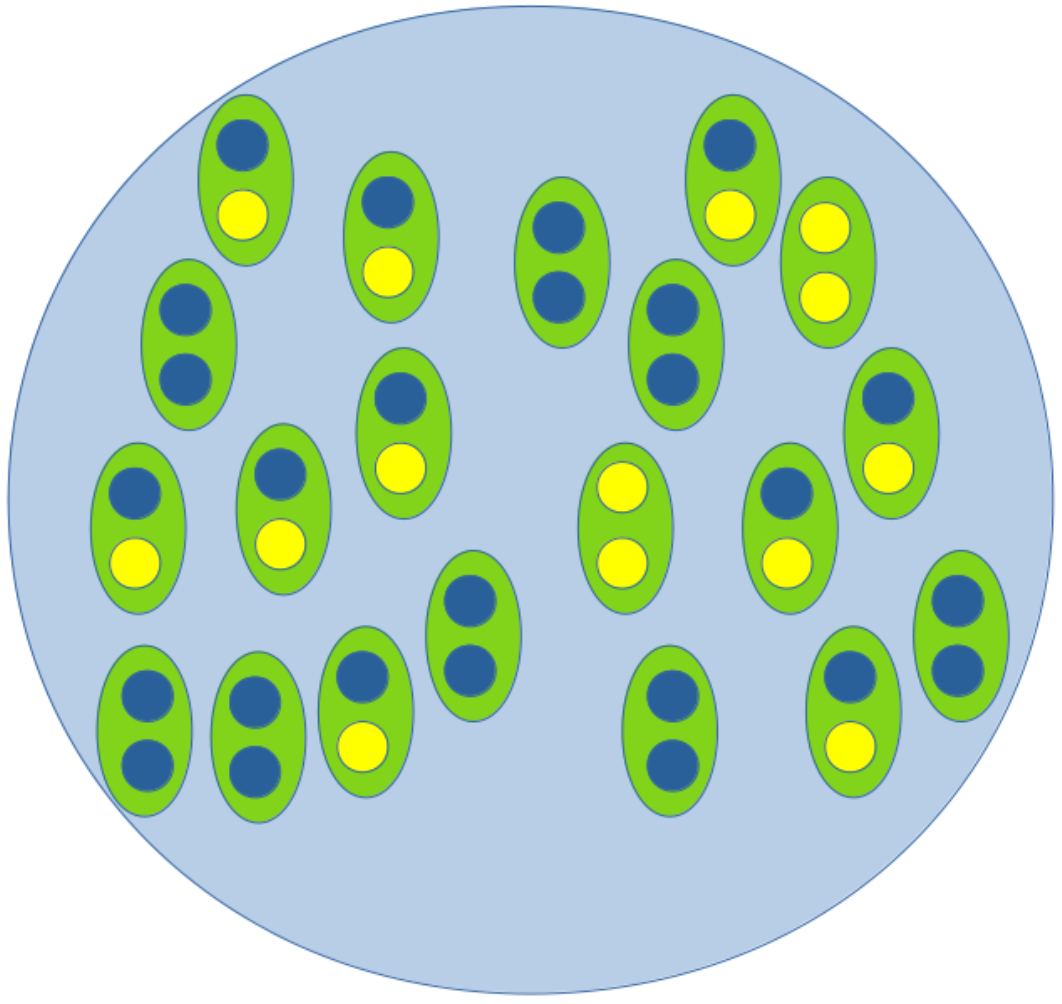
\includegraphics[width=.45\textwidth]{graphics_day2a_popgen/structure_panmictic.png}
	\end{center}
\end{frame}
%%%%%%%%%%%%%%%%%%%%%%%%%%%%%%%%%%%%%%%%%%%%%%%%%%%%%%%%%%%%%%%%%%%%%%%%%%%%%%%%%%%%%%
%
%
%
%%%%%%%%%%%%%%%%%%%%%%%%%%%%%%%%%%%%%%%%%%%%%%%%%%%%%%%%%%%%%%%%%%%%%%%%%%%%%%%%%%%%%
\begin{frame}\frametitle{Population subdivision}
	At some point in time, a geographical/social barrier (dashed line in the figure) may prevent mating between individuals belonging to the two different groups/regions (left and right of the dashed line).
	\begin{center}
		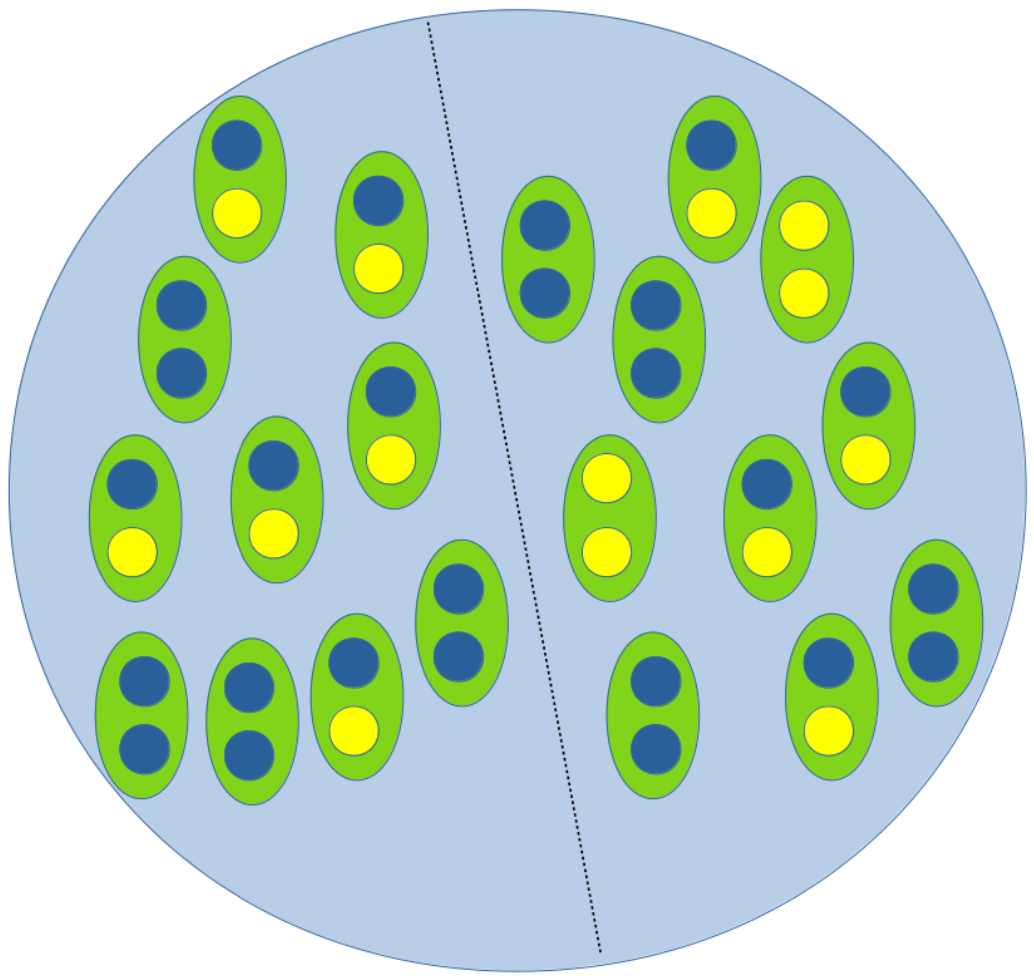
\includegraphics[width=.45\textwidth]{graphics_day2a_popgen/structure_divided.png}
	\end{center}
\end{frame}
%%%%%%%%%%%%%%%%%%%%%%%%%%%%%%%%%%%%%%%%%%%%%%%%%%%%%%%%%%%%%%%%%%%%%%%%%%%%%%%%%%%%%%
%
%
%
%%%%%%%%%%%%%%%%%%%%%%%%%%%%%%%%%%%%%%%%%%%%%%%%%%%%%%%%%%%%%%%%%%%%%%%%%%%%%%%%%%%%%
\begin{frame}\frametitle{Population subdivision}
	The two populations will experience separate genetic drifts and their allele frequency will change independently.
	\begin{center}
		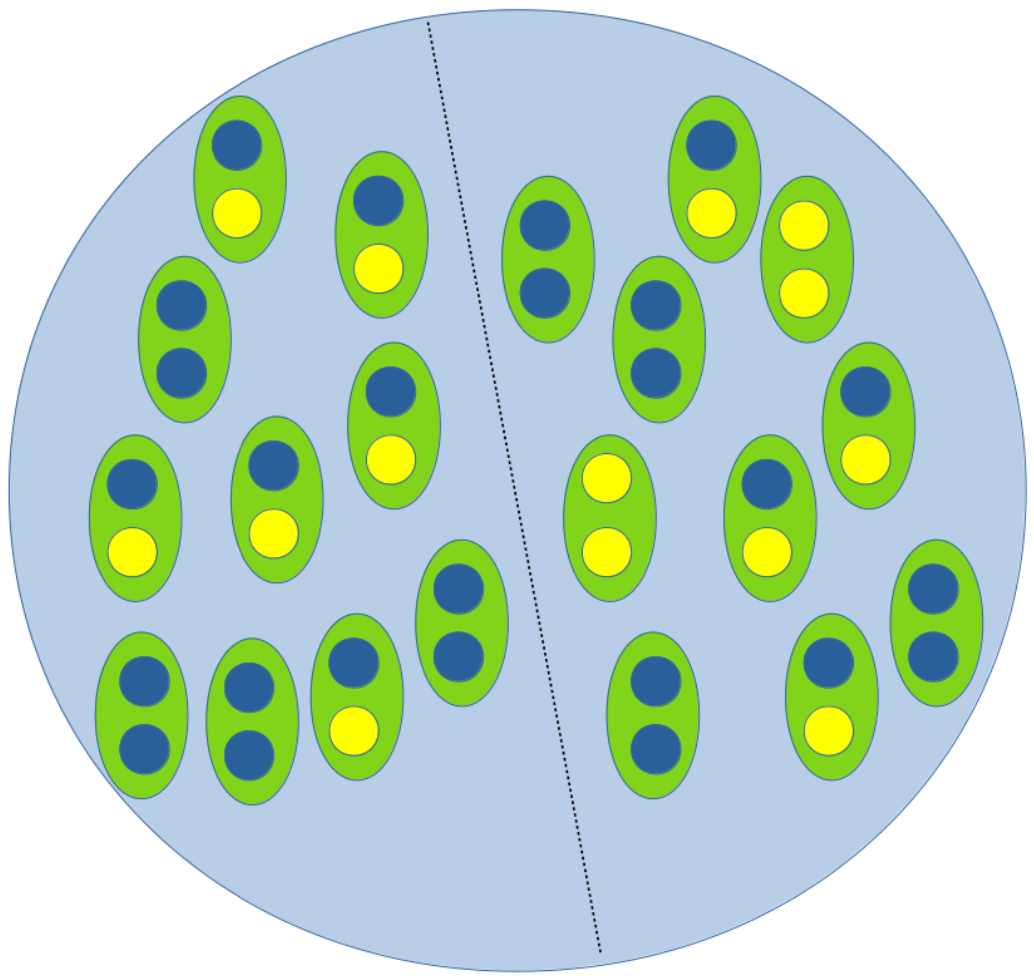
\includegraphics[width=.45\textwidth]{graphics_day2a_popgen/structure_divided.png}
	\end{center}
	What if some individuals can move from one population to another? What will the effect on the allele frequency be?
\end{frame}
%%%%%%%%%%%%%%%%%%%%%%%%%%%%%%%%%%%%%%%%%%%%%%%%%%%%%%%%%%%%%%%%%%%%%%%%%%%%%%%%%%%%%%
%
%
%
%%%%%%%%%%%%%%%%%%%%%%%%%%%%%%%%%%%%%%%%%%%%%%%%%%%%%%%%%%%%%%%%%%%%%%%%%%%%%%%%%%%%%
\begin{frame}
	The model of genetic drift can be extended to include the effect of migration (and therefore of gene flow) and the allele frequency will change accordingly.
	\begin{figure}
	\begin{center}
		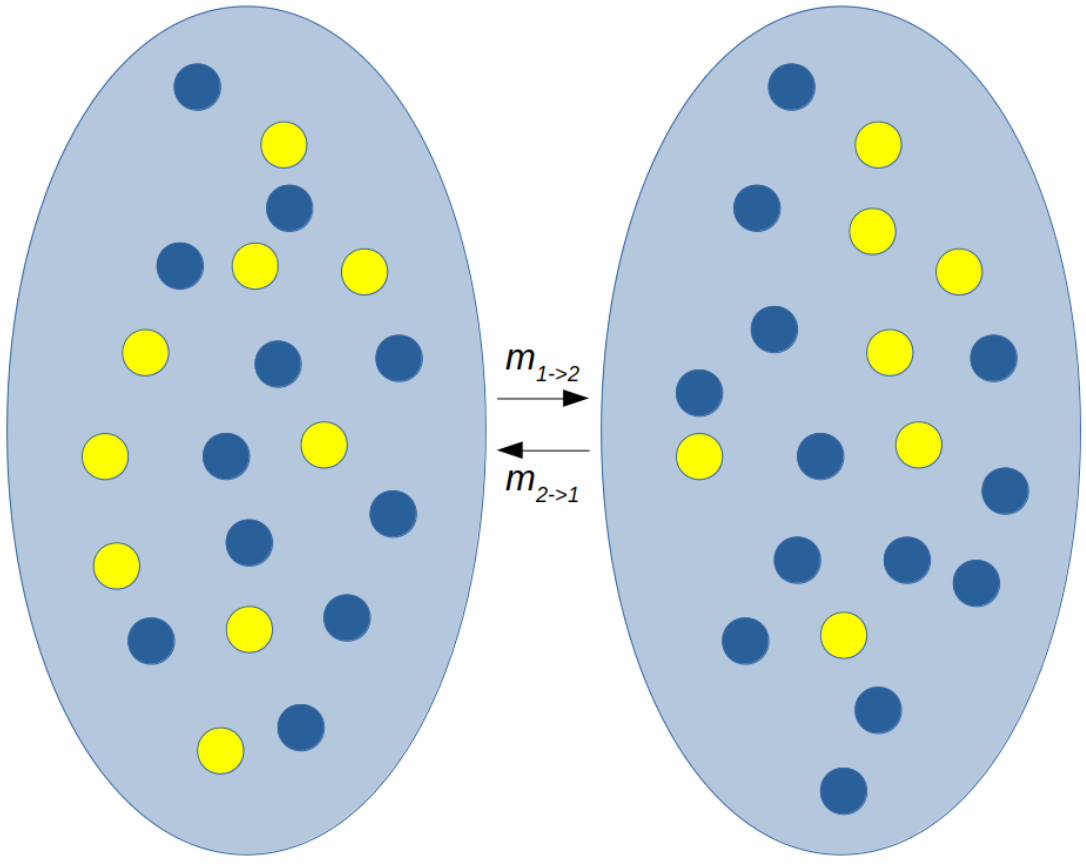
\includegraphics[width=.45\textwidth]{graphics_day2a_popgen/rates_gene_flow.png}
	\end{center}
	\caption{An individual from one population is replaced with an individual from the other with probability $m$ (migration rate).}
	\end{figure}
\end{frame}
%%%%%%%%%%%%%%%%%%%%%%%%%%%%%%%%%%%%%%%%%%%%%%%%%%%%%%%%%%%%%%%%%%%%%%%%%%%%%%%%%%%%%%
%
%
%
%%%%%%%%%%%%%%%%%%%%%%%%%%%%%%%%%%%%%%%%%%%%%%%%%%%%%%%%%%%%%%%%%%%%%%%%%%%%%%%%%%%%%
\begin{frame}
	The model of genetic drift can include gene flow.
	\begin{center}
		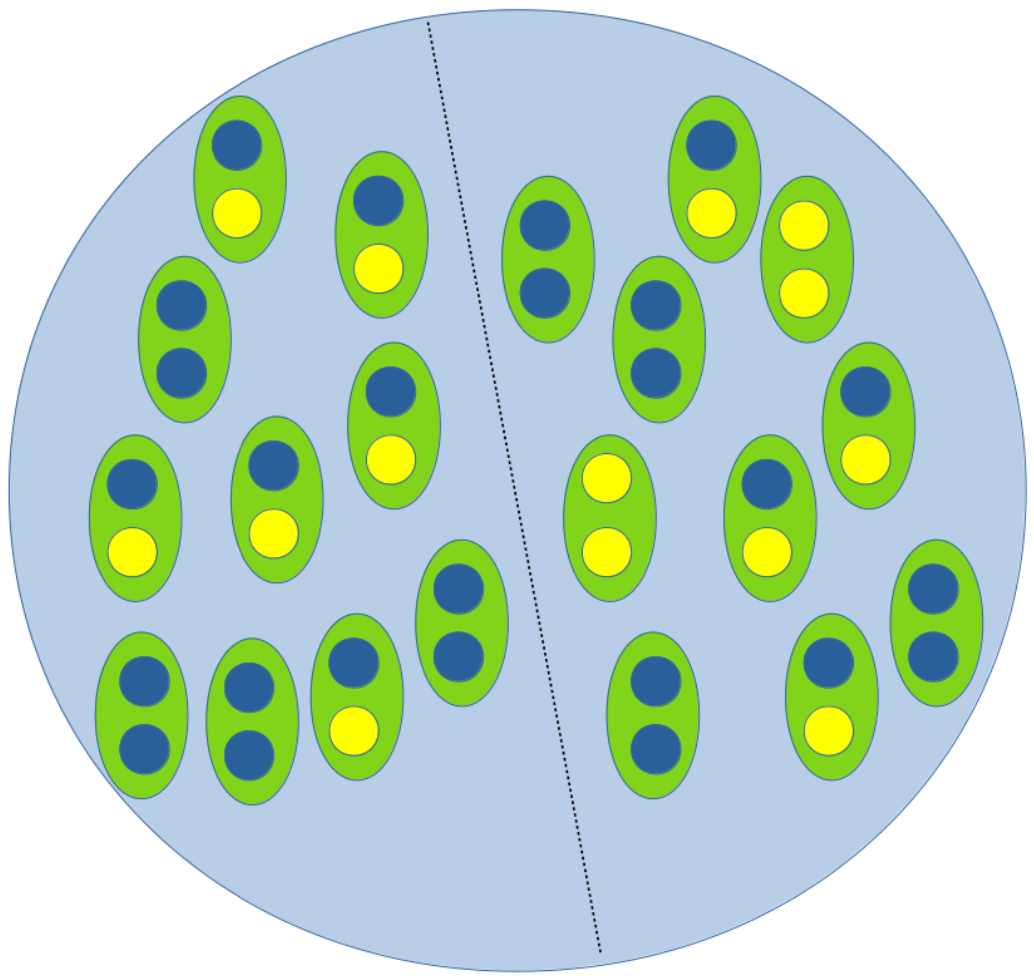
\includegraphics[width=.45\textwidth]{graphics_day2a_popgen/structure_divided.png}
	\end{center}
\end{frame}
%%%%%%%%%%%%%%%%%%%%%%%%%%%%%%%%%%%%%%%%%%%%%%%%%%%%%%%%%%%%%%%%%%%%%%%%%%%%%%%%%%%%%%
%
%
%
%%%%%%%%%%%%%%%%%%%%%%%%%%%%%%%%%%%%%%%%%%%%%%%%%%%%%%%%%%%%%%%%%%%%%%%%%%%%%%%%%%%%%
\begin{frame}\frametitle{Intended Learning Outcomes}
	In this session you have learnt
	\begin{itemize}
		\item To describe all different types of natural selection.
		\item To appreciate the effect of novel mutations on allele frequency.
		\item To understand the concept of gene flow.
	\end{itemize}
\end{frame}
%%%%%%%%%%%%%%%%%%%%%%%%%%%%%%%%%%%%%%%%%%%%%%%%%%%%%%%%%%%%%%%%%%%%%%%%%%%%%%%%%%%%%%
%
%
%
%%%%%%%%%%%%%%%%%%%%%%%%%%%%%%%%%%%%%%%%%%%%%%%%%%%%%%%%%%%%%%%%%%%%%%%%%%%%%%%%%%%%%%
\end{document}
